\documentclass[11pt]{book}
\usepackage{pgfplots}
\usepackage{tikz}
\usepackage{graphicx}
\usepackage{color, colortbl}
\usepackage{comment}
\usepackage{float}
\usepackage{pgfplotstable}
\usepackage{filecontents}




\usepackage{tikz}
\usetikzlibrary{positioning, pgfplots.groupplots}
\usepackage{pgfplots}
\pgfplotsset{compat=newest}
\usepgfplotslibrary{fillbetween}


\usepackage{amsmath,amssymb,amsfonts}
\usepgfplotslibrary{fillbetween}
\usetikzlibrary{pgfplots.fillbetween}
%\usepgfplotslibrary{external}
%\tikzexternalize

\usetikzlibrary{
        matrix, fillbetween
    }



\pgfplotsset{compat=1.6}
\pgfrealjobname{myfile}


% https://tex.stackexchange.com/questions/84127/correctly-align-vertical-text-on-a-baseline-in-pgfplots
\def\mystrut{\vphantom{hg}}

% https://tex.stackexchange.com/questions/204395/add-custom-entry-into-legend-in-pgfplot
\pgfplotsset{
    legend image with text/.style={
        legend image code/.code={%
            \node[anchor=center] at (0.3cm,0cm) {#1};
        }
    },
}




\begin{document}


\beginpgfgraphicnamed{g1}%


\begin{tikzpicture}
 \begin{axis}[
    xmode=log,
    legend style={draw=none},
    legend columns=1,
    legend style={at={(0.97,0.97)}, anchor=north east},
    xmin=1,
    ymin =0.6,
    xmax=4000,
    x dir = reverse,
    xlabel = z,
    ylabel = {\(\rm \rho_B(z)/\rho_B^{ad}(z) = [f_{D}(z)]^{\beta+1}\)}]
  \addplot+[black,mark=none,domain=10:4e3,style={solid} ]
  table[x=z,y=fMF]
  {d/Xe_Recfast++.Rec_corrs_CT2010.PMF_heating.turb.ambi.PF_Lorentz.B0_0.100.Tr.dat};
  \addplot+[red,mark=none,domain=10:4e3,style={solid} ]
  table[x=z,y=fMF]
  {d/Xe_Recfast++.Rec_corrs_CT2010.PMF_heating.turb.ambi.PF_Lorentz.B0_0.500.Tr.dat};
  \addplot+[cyan,mark=none,domain=10:4e3,style={solid} ]
  table[x=z,y=fMF]
  {d/Xe_Recfast++.Rec_corrs_CT2010.PMF_heating.turb.ambi.nonhelical.B0_1.000_nB_2.9.Tr.dat};
  \addplot+[green,mark=none,domain=10:4e3,style={solid} ]
  table[x=z,y=fMF]
  {d/Xe_Recfast++.Rec_corrs_CT2010.PMF_heating.turb.ambi.PF_Lorentz.B0_3.000.Tr.dat};
\addplot +[red,mark=none,dotted] coordinates {(6.0,0.67) (4.0e3,0.67)};
\addplot +[red,mark=none,dotted] coordinates {(8.0,0.684) (4.0e3,0.684)};
\addplot +[red,mark=none,dotted] coordinates {(6.0,0.67) (6.0,0.6)};
\addplot +[red,mark=none,dotted] coordinates {(8.0,0.684) (8.0,0.6)};
\addplot +[red,mark=*] coordinates {(6.0,0.67) (8.0,0.684)};
\legend{$B_0 = 0.1\, nG$, $B_0 = 0.5\, nG$,  $B_0 = 1.0\, nG$,  $B_0 = 3.0\, nG$}
  \end{axis}
\end{tikzpicture}



\endpgfgraphicnamed

\beginpgfgraphicnamed{g2}%


\begin{tikzpicture}
\footnotesize
 \begin{axis}[
    xmode=log,
    legend columns=2,
        legend style={
                    % the /tikz/ prefix is necessary here...
                    % otherwise, it might end-up with `/pgfplots/column 2`
                    % which is not what we want. compare pgfmanual.pdf
            /tikz/column 2/.style={
                column sep=5pt,
            },
        },
%    legend style={draw=none},
%    legend columns=1,
    legend style={at={(0.97,0.97)}, anchor=north east, draw=none},
    xmin=6,
    ymin =0.01,
    ymax=1.19,
    xmax=2000,
    x dir = reverse,
    xlabel = z,
    ylabel = {\(\rm \rho_B(z)/\rho_B^{ad}(z) = [f_{D}(z)]^{\beta+1}\)}]
  \addplot+[black,mark=none,domain=10:4e3,style={solid} ]
  table[x=z,y=fMF]
  {f/Xe_Recfast++.Rec_corrs_CT2010.PMF_heating.turb.ambi.nonhelical.B0_1.000_nB_2.9.Tr.dat};
  \addlegendentry{}‎
  \addplot+[black,mark=none,domain=10:4e3,style={dashed} ]
  table[x=z,y=fMF]
  {f/Xe_Recfast++.Rec_corrs_CT2010.PMF_heating.turb.ambi.helical.B0_1.000_nB_2.9.Tr.dat};
  \addlegendentry{$n_B = -2.9$}
  \addplot+[red,mark=none,domain=10:4e3,style={solid} ]
  table[x=z,y=fMF]
  {f/Xe_Recfast++.Rec_corrs_CT2010.PMF_heating.turb.ambi.nonhelical.B0_1.000_nB_2.0.Tr.dat};
   \addlegendentry{}‎
  \addplot+[red,mark=none,domain=10:4e3,style={dashed} ]
  table[x=z,y=fMF]
  {f/Xe_Recfast++.Rec_corrs_CT2010.PMF_heating.turb.ambi.helical.B0_1.000_nB_2.0.Tr.dat};
   \addlegendentry{$n_B = -2.0$}‎
  \addplot+[blue,mark=none,domain=10:4e3,style={solid} ]
  table[x=z,y=fMF]
  {f/Xe_Recfast++.Rec_corrs_CT2010.PMF_heating.turb.ambi.nonhelical.B0_1.000_nB_1.0.Tr.dat};
   \addlegendentry{}‎
  \addplot+[blue,mark=none,domain=10:4e3,style={dashed} ]
  table[x=z,y=fMF]
  {f/Xe_Recfast++.Rec_corrs_CT2010.PMF_heating.turb.ambi.helical.B0_1.000_nB_1.0.Tr.dat};
   \addlegendentry{$n_B = -1.0$}‎
  \addplot+[green,mark=none,domain=10:4e3,style={solid} ]
  table[x=z,y=fMF]
  {f/Xe_Recfast++.Rec_corrs_CT2010.PMF_heating.turb.ambi.nonhelical.B0_1.000_nB_0.0.Tr.dat};
   \addlegendentry{}‎
   \addplot+[green,mark=none,domain=10:4e3,style={dashed} ]
  table[x=z,y=fMF]
  {f/Xe_Recfast++.Rec_corrs_CT2010.PMF_heating.turb.ambi.helical.B0_1.000_nB_0.0.Tr.dat};
   \addlegendentry{$n_B = -0.0$}‎
%\addplot +[red,mark=none,dotted] coordinates {(6.0,0.67) (4.0e3,0.67)};
%\addplot +[red,mark=none,dotted] coordinates {(8.0,0.684) (4.0e3,0.684)};
%\addplot +[red,mark=none,dotted] coordinates {(6.0,0.67) (6.0,0.6)};
%\addplot +[red,mark=none,dotted] coordinates {(8.0,0.684) (8.0,0.6)};
%\addplot +[red,mark=*] coordinates {(6.0,0.67) (8.0,0.684)};
%\legend{$n_B = -2.9$, $n_B = -2.0$,  $n_B = -1.0$,  $n_B = 0.0$}
\node[] at (axis cs: 700, 1.1) {B$_0$ = 1 nG};
  \end{axis}
\end{tikzpicture}



\endpgfgraphicnamed






\beginpgfgraphicnamed{g3}%




\begin{tikzpicture}
\footnotesize
 \begin{loglogaxis}[
    legend columns=2,
        legend style={
                /tikz/column 2/.style={
                column sep=5pt,
            },
        },
    legend style={draw=none},
    legend style={at={(0.03,0.03)}, anchor=south west},
    xmin=6,
    xmax=4000,
    x dir = reverse,
    xlabel = z,
    ylabel = {\(\rm T_K, T_R\)}]


  \addplot+[orange,mark=none,domain=10:4e3,style={solid} ]
  table[x=z,y=TM]
  {f/Xe_Recfast++.Rec_corrs_CT2010.PMF_heating.turb.ambi.nonhelical.B0_3.000_nB_2.9.Tr.dat}; \label{pgfplots:c1r1}
  \addlegendentry{}‎
  \addplot+[orange,mark=none,domain=10:4e3,style={dashed} ]
  table[x=z,y=TM]
  {f/Xe_Recfast++.Rec_corrs_CT2010.PMF_heating.turb.ambi.helical.B0_3.000_nB_2.9.Tr.dat}; \label{pgfplots:c2r1}
  \addlegendentry{$B_0 = 3.0\, \textrm{nG}$}
  \addplot+[blue,mark=none,domain=10:4e3,style={solid} ]
  table[x=z,y=TM]
  {f/Xe_Recfast++.Rec_corrs_CT2010.PMF_heating.turb.ambi.nonhelical.B0_1.000_nB_2.9.Tr.dat}; \label{pgfplots:c1r2}
  \addlegendentry{}‎
  \addplot+[blue,mark=none,domain=10:4e3,style={dashed} ]
  table[x=z,y=TM]
  {f/Xe_Recfast++.Rec_corrs_CT2010.PMF_heating.turb.ambi.helical.B0_1.000_nB_2.9.Tr.dat}; \label{pgfplots:c2r2}
  \addlegendentry{$B_0 = 1.0\, \textrm{nG}$}
  \addplot+[green,mark=none,domain=10:4e3,style={solid} ]
  table[x=z,y=TM]
  {f/Xe_Recfast++.Rec_corrs_CT2010.PMF_heating.turb.ambi.nonhelical.B0_0.500_nB_2.9.Tr.dat}; \label{pgfplots:c1r3}
  \addlegendentry{}‎
  \addplot+[green,mark=none,domain=10:4e3,style={dashed} ]
  table[x=z,y=TM]
  {f/Xe_Recfast++.Rec_corrs_CT2010.PMF_heating.turb.ambi.helical.B0_0.500_nB_2.9.Tr.dat}; \label{pgfplots:c2r3}
  \addlegendentry{$B_0 = 0.5\, \textrm{nG}$}
  \addplot+[cyan,mark=none,domain=10:4e3,style={solid} ]
  table[x=z,y=TM]
  {f/Xe_Recfast++.Rec_corrs_CT2010.PMF_heating.turb.ambi.nonhelical.B0_0.100_nB_2.9.Tr.dat}; \label{pgfplots:c1r4}
  \addlegendentry{}‎
  \addplot+[cyan,mark=none,domain=10:4e3,style={dashed} ]
  table[x=z,y=TM]
  {f/Xe_Recfast++.Rec_corrs_CT2010.PMF_heating.turb.ambi.helical.B0_0.100_nB_2.9.Tr.dat}; \label{pgfplots:c2r4}
  \addlegendentry{$B_0 = 0.1\, \textrm{nG}$}


       \addlegendimage{legend image with text=${}$}
        \addlegendentry{}
  \addplot+[black,mark=none,domain=10:4e3,style={solid} ]
  table[x=z,y=TM]
  {f/Xe_Recfast++.Rec_corrs_CT2010.dat}; \label{pgfplots:c2r5}
  \addlegendentry{$B_0 = 0.0\, \textrm{nG}$}


     \addlegendimage{legend image with text=${}$}
        \addlegendentry{}
  \addplot+[red,mark=none,domain=6:4e3,style={dashed, line width=0.9pt}]
		{2.72548*(1+x)}; \label{pgfplots:c2r5}
				\addlegendentry{$T_R$}
% \legend{$B_0 = 0.0\, nG$, $B_0 = 0.1\, nG$, $B_0 = 0.5\, nG$,  $B_0 = 1.0\, nG$,  $B_0 = 3.0\, nG$, CMB}
\node[] at (axis cs: 1500, 120) {$n_B = -2.9$};
  \end{loglogaxis}

\end{tikzpicture}

\endpgfgraphicnamed








\beginpgfgraphicnamed{g4}%

\begin{tikzpicture}
\footnotesize
 \begin{loglogaxis}[
 name=plot1,
    title= 'H'-subsystem,
    legend columns=5,
    legend style={at={(1.0,0.02)}, anchor=south east, nodes={scale=0.7, transform shape}},
    legend style={draw=none, fill=none},
    legend cell align={left},
    xmin=10,
    xmax=4000,
    ymin = 1e-30,
    x dir = reverse,
    xlabel = z,
    ylabel = {\(\rm \textcolor{blue}{X_{H_2^+}},\, \textcolor{cyan}{X_{H^-}},\, \textcolor{red}{X_{H_2}},\, \textcolor{green}{X_{H}},\, X_{H^+}\)}]

  \addplot+[black,mark=none,domain=10:4e3,style={dashed} ]
  table[x=z,y=p]
  {f/Xe_Recfast++.Rec_corrs_CT2010.PMF_heating.turb.ambi.nonhelical.B0_1.000_nB_2.9.Tr.dat};
  \addplot+[red,mark=none,domain=10:4e3,style={dashed} ]
  table[x=z,y=H2]
  {f/Xe_Recfast++.Rec_corrs_CT2010.PMF_heating.turb.ambi.nonhelical.B0_1.000_nB_2.9.Tr.dat};
  \addplot+[cyan,mark=none,domain=10:4e3,style={dashed} ]
  table[x=z,y=H2p]
  {f/Xe_Recfast++.Rec_corrs_CT2010.PMF_heating.turb.ambi.nonhelical.B0_1.000_nB_2.9.Tr.dat};
 \addplot+[green,mark=none,domain=10:4e3,style={dashed} ]
  table[x=z,y=H]
  {f/Xe_Recfast++.Rec_corrs_CT2010.PMF_heating.turb.ambi.nonhelical.B0_1.000_nB_2.9.Tr.dat};
  \addplot+[blue,mark=none,domain=10:4e3,style={dashed} ]
  table[x=z,y=Hm]
  {f/Xe_Recfast++.Rec_corrs_CT2010.PMF_heating.turb.ambi.nonhelical.B0_1.000_nB_2.9.Tr.dat};
  \addplot+[black,mark=none,domain=10:4e3,style={dotted}, line width=0.8pt ]
  table[x=z,y=p]
  {f/Xe_Recfast++.Rec_corrs_CT2010.PMF_heating.turb.ambi.helical.B0_1.000_nB_2.9.Tr.dat};
  \addplot+[red,mark=none,domain=10:4e3,style={dotted}, line width=0.8pt ]
  table[x=z,y=H2]
  {f/Xe_Recfast++.Rec_corrs_CT2010.PMF_heating.turb.ambi.helical.B0_1.000_nB_2.9.Tr.dat};
  \addplot+[cyan,mark=none,domain=10:4e3,style={dotted}, line width=0.8pt ]
  table[x=z,y=H2p]
  {f/Xe_Recfast++.Rec_corrs_CT2010.PMF_heating.turb.ambi.helical.B0_1.000_nB_2.9.Tr.dat};
 \addplot+[green,mark=none,domain=10:4e3,style={dotted}, line width=0.8pt ]
  table[x=z,y=H]
  {f/Xe_Recfast++.Rec_corrs_CT2010.PMF_heating.turb.ambi.helical.B0_1.000_nB_2.9.Tr.dat};
  \addplot+[blue,mark=none,domain=10:4e3,style={dotted}, line width=0.8pt ]
  table[x=z,y=Hm]
  {f/Xe_Recfast++.Rec_corrs_CT2010.PMF_heating.turb.ambi.helical.B0_1.000_nB_2.9.Tr.dat};

    \addplot+[black,mark=none,domain=10:4e3,style={solid} ]
  table[x=z,y=p]
    {f/Xe_Recfast++.Rec_corrs_CT2010.dat};
  \addplot+[red,mark=none,domain=10:4e3,style={solid} ]
  table[x=z,y=H2]
    {f/Xe_Recfast++.Rec_corrs_CT2010.dat};
  \addplot+[cyan,mark=none,domain=10:4e3,style={solid} ]
  table[x=z,y=H2p]
    {f/Xe_Recfast++.Rec_corrs_CT2010.dat};
  \addplot+[green,mark=none,domain=10:4e3,style={solid} ]
  table[x=z,y=H]
    {f/Xe_Recfast++.Rec_corrs_CT2010.dat};
  \addplot+[blue,mark=none,domain=10:4e3,style={solid} ]
  table[x=z,y=Hm]
  {f/Xe_Recfast++.Rec_corrs_CT2010.dat};

 % \node[] at (axis cs: 20, 1.e-20) {\bf B$_0$ = 1 nG};
    \legend{$\,$,$\,$,$\,$, $\,$, {\bf
    $\begin{array}[b]{l}
      {\bf B_0 = 1\, nG}\\
      {\rm\bf (nonhelical)}
      \end{array}$},
            $\,$,$\,$,$\,$, $\,$, {\bf
    $\begin{array}[b]{l}
      {\bf B_0 = 1\, nG}\\
      {\rm\bf (helical)}
      \end{array}$},
            $\,$,$\,$,$\,$, $\,$, {\bf
    $\begin{array}[b]{l}
      {\bf B_0 = 0\, nG}
      \end{array}$}}
  \end{loglogaxis}
%\end{tikzpicture}
%\begin{tikzpicture}

%\end{tikzpicture}
%\begin{tikzpicture}
 \begin{loglogaxis}[
 name=plot3,
at=(plot1.below south east), anchor=above north east,
    title= 'He'-subsystem,
    legend columns=3,
    legend style={at={(0.97,0.03)}, anchor=south east},
    legend style={draw=none, fill opacity=0.7},
    xmin=10,
    xmax=4000,
    ymin = 1e-30,
    x dir = reverse,
    xlabel = z,
    ylabel = {\(\rm \textcolor{green}{X_{He}},\, \textcolor{red}{X_{HeH^+}},\, X_{He^+}\)}]

  \addplot+[black,mark=none,domain=10:4e3,style={dashed} ]
  table[x=z,y=Hep]
  {f/Xe_Recfast++.Rec_corrs_CT2010.PMF_heating.turb.ambi.nonhelical.B0_1.000_nB_2.9.Tr.dat};
  \addplot+[red,mark=none,domain=10:4e3,style={dashed} ]
  table[x=z,y=HeHp]
  {f/Xe_Recfast++.Rec_corrs_CT2010.PMF_heating.turb.ambi.nonhelical.B0_1.000_nB_2.9.Tr.dat};
  \addplot+[green,mark=none,domain=10:4e3,style={dashed} ]
  table[x=z,y=He]
  {f/Xe_Recfast++.Rec_corrs_CT2010.PMF_heating.turb.ambi.nonhelical.B0_1.000_nB_2.9.Tr.dat};


  \addplot+[black,mark=none,domain=10:4e3,style={dotted}, line width=0.8pt ]
  table[x=z,y=Hep]
  {f/Xe_Recfast++.Rec_corrs_CT2010.PMF_heating.turb.ambi.helical.B0_1.000_nB_2.9.Tr.dat};
  \addplot+[red,mark=none,domain=10:4e3,style={dotted}, line width=0.8pt ]
  table[x=z,y=HeHp]
  {f/Xe_Recfast++.Rec_corrs_CT2010.PMF_heating.turb.ambi.helical.B0_1.000_nB_2.9.Tr.dat};
  \addplot+[green,mark=none,domain=10:4e3,style={dotted}, line width=0.8pt ]
  table[x=z,y=He]
  {f/Xe_Recfast++.Rec_corrs_CT2010.PMF_heating.turb.ambi.helical.B0_1.000_nB_2.9.Tr.dat};

    \addplot+[black,mark=none,domain=10:4e3,style={solid}]
  table[x=z,y=Hep]
    {f/Xe_Recfast++.Rec_corrs_CT2010.dat};
  %{f/Xe_Recfast++.Rec_corrs_CT2010.dat};
  \addplot+[red,mark=none,domain=10:4e3,style={solid} ]
  table[x=z,y=HeHp]
    {f/Xe_Recfast++.Rec_corrs_CT2010.dat};
  %{f/Xe_Recfast++.Rec_corrs_CT2010.dat};
  \addplot+[green,mark=none,domain=10:4e3,style={solid} ]
  table[x=z,y=He]
    {f/Xe_Recfast++.Rec_corrs_CT2010.dat};
  %{f/Xe_Recfast++.Rec_corrs_CT2010.dat};


%  \legend{$\,$,$\,$, $B_0 = 1\, \textrm{nG}$,
%            $\,$,$\,$, $B_0 = 1\, \textrm{nG}$,
%            $\,$,$\,$, $B_0 = 0\, \textrm{nG}$}
 \end{loglogaxis}
%\end{tikzpicture}
%\begin{tikzpicture}
 \begin{loglogaxis}[
 name=plot4,
at=(plot3.right of north east), anchor=left of north west,
    title= Formation of the first molecules,
    legend columns=4,
    legend style={at={(0.97,0.03)}, anchor=south east},
    legend style={draw=none, fill opacity=0.7},
    xmin=10,
    xmax=4000,
    ymin = 1e-30,
    x dir = reverse,
    xlabel = z,
    ylabel = {\(\rm \textcolor{blue}{X_{HeH^+}},\, \textcolor{green}{X_{HD}},\, \textcolor{red}{X_{H_2}},\, X_{H^+}\)}]


  \addplot+[black,mark=none,domain=10:4e3,style={dashed} ]
  table[x=z,y=p]
  {f/Xe_Recfast++.Rec_corrs_CT2010.PMF_heating.turb.ambi.nonhelical.B0_1.000_nB_2.9.Tr.dat};
  \addplot+[red,mark=none,domain=10:4e3,style={dashed} ]
  table[x=z,y=H2]
  {f/Xe_Recfast++.Rec_corrs_CT2010.PMF_heating.turb.ambi.nonhelical.B0_1.000_nB_2.9.Tr.dat};
  \addplot+[green,mark=none,domain=10:4e3,style={dashed} ]
  table[x=z, y expr=\thisrow{HD}*2.614e-5]
  {f/Xe_Recfast++.Rec_corrs_CT2010.PMF_heating.turb.ambi.nonhelical.B0_1.000_nB_2.9.Tr.dat};
  \addplot+[blue,mark=none,domain=10:4e3,style={dashed} ]
  table[x=z, y expr=\thisrow{HeHp}*0.0795134]
  {f/Xe_Recfast++.Rec_corrs_CT2010.PMF_heating.turb.ambi.nonhelical.B0_1.000_nB_2.9.Tr.dat};

  \addplot+[black,mark=none,domain=10:4e3,style={dotted} ]
  table[x=z,y=p]
  {f/Xe_Recfast++.Rec_corrs_CT2010.PMF_heating.turb.ambi.helical.B0_1.000_nB_2.9.Tr.dat};
  \addplot+[red,mark=none,domain=10:4e3,style={dotted} ]
  table[x=z,y=H2]
  {f/Xe_Recfast++.Rec_corrs_CT2010.PMF_heating.turb.ambi.helical.B0_1.000_nB_2.9.Tr.dat};
  \addplot+[green,mark=none,domain=10:4e3,style={dotted} ]
  table[x=z, y expr=\thisrow{HD}*2.614e-5]
  {f/Xe_Recfast++.Rec_corrs_CT2010.PMF_heating.turb.ambi.helical.B0_1.000_nB_2.9.Tr.dat};
  \addplot+[blue,mark=none,domain=10:4e3,style={dotted} ]
  table[x=z, y expr=\thisrow{HeHp}*0.0795134]
  {f/Xe_Recfast++.Rec_corrs_CT2010.PMF_heating.turb.ambi.helical.B0_1.000_nB_2.9.Tr.dat};


  \addplot+[black,mark=none,domain=10:4e3,style={solid} ]
  table[x=z,y=p]
    {f/Xe_Recfast++.Rec_corrs_CT2010.dat};
%  {f/Xe_Recfast++.Rec_corrs_CT2010.dat};
  \addplot+[red,mark=none,domain=10:4e3,style={solid} ]
  table[x=z,y=H2]
    {f/Xe_Recfast++.Rec_corrs_CT2010.dat};
%  {f/Xe_Recfast++.Rec_corrs_CT2010.dat};
  \addplot+[green,mark=none,domain=10:4e3,style={solid}]
  table[x=z, y expr=\thisrow{HD}*2.614e-5]
    {f/Xe_Recfast++.Rec_corrs_CT2010.dat};
%  {f/Xe_Recfast++.Rec_corrs_CT2010.dat};
  \addplot+[blue,mark=none,domain=10:4e3,style={solid} ]
  table[x=z, y expr=\thisrow{HeHp}*0.0795134]
    {f/Xe_Recfast++.Rec_corrs_CT2010.dat};
%  {f/Xe_Recfast++.Rec_corrs_CT2010.dat};

%   \legend{$\,$,$\,$, $\,$, $B_0 = 1\, \textrm{nG}$,
%           $\,$,$\,$, $\,$, $B_0 = 1\, \textrm{nG}$,
%            $\,$,$\,$, $\,$, $B_0 = 0\, \textrm{nG}$}
 \end{loglogaxis}
  \begin{loglogaxis}[
 name=plot2,
at=(plot4.above north west), anchor=below south west,
    title= 'D'-subsystem,
    legend columns=3,
    legend style={at={(0.97,0.03)}, anchor=south east},
    legend style={draw=none, fill opacity=0.7},
    xmin=10,
    xmax=4000,
    ymin = 1e-30,
    x dir = reverse,
    xlabel = z,
    ylabel = {\(\rm \textcolor{green}{X_{D}},\, \textcolor{red}{X_{HD}},\, X_{D^+}\)}]

  \addplot+[black,mark=none,domain=10:4e3,style={dashed} ]
  table[x=z,y=Dp]
  {f/Xe_Recfast++.Rec_corrs_CT2010.PMF_heating.turb.ambi.nonhelical.B0_1.000_nB_2.9.Tr.dat};
  \addplot+[red,mark=none,domain=10:4e3,style={dashed} ]
  table[x=z,y=HD]
  {f/Xe_Recfast++.Rec_corrs_CT2010.PMF_heating.turb.ambi.nonhelical.B0_1.000_nB_2.9.Tr.dat};
  \addplot+[green,mark=none,domain=10:4e3,style={dashed} ]
  table[x=z,y=D]
  {f/Xe_Recfast++.Rec_corrs_CT2010.PMF_heating.turb.ambi.nonhelical.B0_1.000_nB_2.9.Tr.dat};


  \addplot+[black,mark=none,domain=10:4e3,style={dotted} ]
  table[x=z,y=Dp]
  {f/Xe_Recfast++.Rec_corrs_CT2010.PMF_heating.turb.ambi.helical.B0_1.000_nB_2.9.Tr.dat};
  \addplot+[red,mark=none,domain=10:4e3,style={dotted} ]
  table[x=z,y=HD]
  {f/Xe_Recfast++.Rec_corrs_CT2010.PMF_heating.turb.ambi.helical.B0_1.000_nB_2.9.Tr.dat};
  \addplot+[green,mark=none,domain=10:4e3,style={dotted} ]
  table[x=z,y=D]
  {f/Xe_Recfast++.Rec_corrs_CT2010.PMF_heating.turb.ambi.helical.B0_1.000_nB_2.9.Tr.dat};


  \addplot+[black,mark=none,domain=10:4e3,style={solid} ]
  table[x=z,y=Dp]
    {f/Xe_Recfast++.Rec_corrs_CT2010.dat};
  %{f/Xe_Recfast++.Rec_corrs_CT2010.dat};
  \addplot+[red,mark=none,domain=10:4e3,style={solid} ]
  table[x=z,y=HD]
    {f/Xe_Recfast++.Rec_corrs_CT2010.dat};
  %{f/Xe_Recfast++.Rec_corrs_CT2010.dat};
  \addplot+[green,mark=none,domain=10:4e3,style={solid} ]
  table[x=z,y=D]
    {f/Xe_Recfast++.Rec_corrs_CT2010.dat};
  %{f/Xe_Recfast++.Rec_corrs_CT2010.dat};

 % \legend{$\,$,$\,$, $B_0 = 1\, \textrm{nG}$,
 %         $\,$,$\,$, $B_0 = 1\, \textrm{nG}$,
 %           $\,$,$\,$, $B_0 = 0\, \textrm{nG}$}
 \end{loglogaxis}
\end{tikzpicture}

\endpgfgraphicnamed


\beginpgfgraphicnamed{g5}%

\begin{tikzpicture}
\footnotesize
 \begin{axis}[
    legend columns=2,
    xmode=log,
    legend style={at={(0.03,0.63)}, anchor=north west},
     legend style={draw=none, fill=none},
    xmin=10,
    xmax=1200,
    x dir = reverse,
    xlabel = z,
    ylabel = {\(\rm \textcolor{red}{n^{para}_{H_2}/n^{tot}_{H_2}},\quad n^{orto}_{H_2}/n^{tot}_{H_2}\)}]
  \addplot+[black,mark=none,domain=10:4e3,style={solid} ]
  table[x=z,y=H2orto]
  {f/Xe_Recfast++.Rec_corrs_CT2010.dat};
  \addplot+[red,mark=none,domain=10:4e3,style={solid} ]
  table[x=z,y=H2para]
  {f/Xe_Recfast++.Rec_corrs_CT2010.dat};
 \addplot+[black,mark=none,domain=10:4e3,style={dotted} ]
  table[x=z,y=H2orto]
  {f/Xe_Recfast++.Rec_corrs_CT2010.PMF_heating.turb.ambi.nonhelical.B0_0.500_nB_2.9.Tr.dat};
  \addplot+[red,mark=none,domain=10:4e3,style={dotted} ]
  table[x=z,y=H2para]
  {f/Xe_Recfast++.Rec_corrs_CT2010.PMF_heating.turb.ambi.nonhelical.B0_0.500_nB_2.9.Tr.dat};
  \addplot+[black,mark=none,domain=10:4e3,style={dashed} ]
  table[x=z,y=H2orto]
  {f/Xe_Recfast++.Rec_corrs_CT2010.PMF_heating.turb.ambi.nonhelical.B0_1.000_nB_2.9.Tr.dat};
  \addplot+[red,mark=none,domain=10:4e3,style={dashed} ]
  table[x=z,y=H2para]
  {f/Xe_Recfast++.Rec_corrs_CT2010.PMF_heating.turb.ambi.nonhelical.B0_1.000_nB_2.9.Tr.dat};

   \legend{$\,$, $B_0 = 0.0\, \textrm{nG}$,
            $\,$, $B_0 = 0.5\, \textrm{nG}$,
            $\,$, $B_0 = 1.0\, \textrm{nG}$}
\end{axis}
\end{tikzpicture}

\endpgfgraphicnamed








\beginpgfgraphicnamed{g6}%

\begin{tikzpicture}
\begin{axis}[
 name=plot1,
xmode=log,
  legend style={draw=none},
%    legend columns=1,
    legend style={at={(0.97,0.97)}, anchor=north east},
%   title= {H$_2$ lines emission for B$_0$ = 3 nG},
%    ymin=1e-2,
    xmin=5,
    xmax=6000,
%    transpose legend,
%    legend columns=-1,
%    legend to name=named,
%    legend style={at={(0.5,-0.2)},anchor=north},
%    legend style={at={(0.97,0.97)}, anchor=north east},
	xlabel=Frequency (GHz),
	ylabel=Spectral Radiance (Jy/sr)]

%	\node[] at (axis cs: 20, 100) {B$_0$ = 3 nG};
\node[] at (axis cs: 10, 0.5) {\bf H$_2$}; %0.85 for B_0 = 3 nG
 \addplot+[black,mark=none,domain=10:4e3,style={solid, line width=1pt} ]
  table[x=F,y=H2_ALL]
  {f/level_occupations_B0_1.000_nB_2.9.nonhelical.dat};
%  \addlegendentry{Total}

  \addplot+[red,mark=none,domain=10:4e3,style={dotted, line width=1pt} ]
  table[x=F,y=H2_20]
  {f/level_occupations_B0_1.000_nB_2.9.nonhelical.dat};
 % \addlegendentry{ 2$\rightarrow$0}

\addplot+[blue,mark=none,domain=10:4e3,style={dotted, line width=1pt} ]
  table[x=F,y=H2_31]
  {f/level_occupations_B0_1.000_nB_2.9.nonhelical.dat};
 % \addlegendentry{3$\rightarrow$1}

\addplot+[green,mark=none,domain=10:4e3,style={dotted, line width=1pt} ]
  table[x=F,y=H2_42]
  {f/level_occupations_B0_1.000_nB_2.9.nonhelical.dat};
 % \addlegendentry{4$\rightarrow$2}

\addplot+[cyan,mark=none,domain=10:4e3,style={dotted, line width=1pt} ]
  table[x=F,y=H2_53]
  {f/level_occupations_B0_1.000_nB_2.9.nonhelical.dat};
%  \addlegendentry{5$\rightarrow$3}

\addplot+[olive,mark=none,domain=10:4e3,style={dotted, line width=1pt} ]
  table[x=F,y=H2_64]
  {f/level_occupations_B0_1.000_nB_2.9.nonhelical.dat};
%  \addlegendentry{6$\rightarrow$4}

\addplot+[teal,mark=none,domain=10:4e3,style={dotted, line width=1pt} ]
  table[x=F,y=H2_75]
  {f/level_occupations_B0_1.000_nB_2.9.nonhelical.dat};
%  \addlegendentry{7$\rightarrow$5}

\addplot+[violet,mark=none,domain=10:4e3,style={dotted, line width=1pt} ]
  table[x=F,y=H2_86]
  {f/level_occupations_B0_1.000_nB_2.9.nonhelical.dat};
%  \addlegendentry{8$\rightarrow$6}
\end{axis}
%\end{tikzpicture}
%\begin{tikzpicture}
\begin{axis}[
 name=plot2,
xmode=log,
   legend style={at={(0.97,0.2)}, anchor=south east},
    legend style={draw=none},
at=(plot1.right of north east), anchor=left of north west,
%   title= {H$_2$ lines emission for B$_0$ = 3 nG},
 %   ymin=1e-2,
    xmin=2,
    xmax=1000,
    x dir = reverse,
	xlabel=redshift,
	ylabel=Spectral Radiance (Jy/sr)]

%	\node[] at (axis cs: 20, 100) {B$_0$ = 3 nG};

 \addplot+[black,mark=none,domain=10:4e3,style={solid, line width=1pt} ]
  table[x=zem,y=H2_ALL]
  {f/level_occupations_z_B0_1.000_nB_2.9.nonhelical.dat};
  \addlegendentry{Total}

  \addplot+[red,mark=none,domain=10:4e3,style={dotted, line width=1pt} ]
  table[x=zem,y=H2_20]
  {f/level_occupations_z_B0_1.000_nB_2.9.nonhelical.dat};
  \addlegendentry{ 2$\rightarrow$0}

\addplot+[blue,mark=none,domain=10:4e3,style={dotted, line width=1pt} ]
  table[x=zem,y=H2_31]
  {f/level_occupations_z_B0_1.000_nB_2.9.nonhelical.dat};
  \addlegendentry{3$\rightarrow$1}

\addplot+[green,mark=none,domain=10:4e3,style={dotted, line width=1pt} ]
  table[x=zem,y=H2_42]
  {f/level_occupations_z_B0_1.000_nB_2.9.nonhelical.dat};
  \addlegendentry{4$\rightarrow$2}

\addplot+[cyan,mark=none,domain=10:4e3,style={dotted, line width=1pt} ]
  table[x=zem,y=H2_53]
  {f/level_occupations_z_B0_1.000_nB_2.9.nonhelical.dat};
  \addlegendentry{5$\rightarrow$3}

\addplot+[olive,mark=none,domain=10:4e3,style={dotted, line width=1pt} ]
  table[x=zem,y=H2_64]
  {f/level_occupations_z_B0_1.000_nB_2.9.nonhelical.dat};
  \addlegendentry{6$\rightarrow$4}

\addplot+[teal,mark=none,domain=10:4e3,style={dotted, line width=1pt} ]
  table[x=zem,y=H2_75]
  {f/level_occupations_z_B0_1.000_nB_2.9.nonhelical.dat};
  \addlegendentry{7$\rightarrow$5}

\addplot+[violet,mark=none,domain=10:4e3,style={dotted, line width=1pt} ]
  table[x=zem,y=H2_86]
  {f/level_occupations_z_B0_1.000_nB_2.9.nonhelical.dat};
  \addlegendentry{8$\rightarrow$6}
\end{axis}

\end{tikzpicture}

\endpgfgraphicnamed



\beginpgfgraphicnamed{g7}%



\begin{tikzpicture}
\begin{axis}[
 name=plot1,
xmode=log,
ylabel shift={2pt},
yticklabel shift={5pt},
  legend style={draw=none},
%    legend columns=1,
    legend style={at={(0.97,0.97)}, anchor=north east},
%   title= {H$_2$ lines emission for B$_0$ = 3 nG},
%    ymin=1e-2,
    xmin=5,
    xmax=6000,
%    transpose legend,
%    legend columns=-1,
%    legend to name=named,
%    legend style={at={(0.5,-0.2)},anchor=north},
%    legend style={at={(0.97,0.97)}, anchor=north east},
	xlabel=Frequency (GHz),
	ylabel=Spectral Radiance (Jy/sr)]

%	\node[] at (axis cs: 20, 50) {B$_0$ = 3 nG};
\node[] at (axis cs: 10, 3.8e-4) {\bf HD}; %5.e-2

 \addplot+[black,mark=none,domain=10:4e3,style={solid, line width=1pt} ]
  table[x=F,y=HD_ALL]
  {f/level_occupations_B0_1.000_nB_2.9.nonhelical.dat};
%  \addlegendentry{Total}

  \addplot+[red,mark=none,domain=10:4e3,style={dotted, line width=1pt} ]
  table[x=F,y=HD_10]
  {f/level_occupations_B0_1.000_nB_2.9.nonhelical.dat};
 % \addlegendentry{ 2$\rightarrow$0}

\addplot+[blue,mark=none,domain=10:4e3,style={dotted, line width=1pt} ]
  table[x=F,y=HD_21]
  {f/level_occupations_B0_1.000_nB_2.9.nonhelical.dat};
 % \addlegendentry{3$\rightarrow$1}

\addplot+[green,mark=none,domain=10:4e3,style={dotted, line width=1pt} ]
  table[x=F,y=HD_32]
  {f/level_occupations_B0_1.000_nB_2.9.nonhelical.dat};
 % \addlegendentry{4$\rightarrow$2}

\addplot+[cyan,mark=none,domain=10:4e3,style={dotted, line width=1pt} ]
  table[x=F,y=HD_43]
  {f/level_occupations_B0_1.000_nB_2.9.nonhelical.dat};
%  \addlegendentry{5$\rightarrow$3}

\addplot+[olive,mark=none,domain=10:4e3,style={dotted, line width=1pt} ]
  table[x=F,y=HD_54]
  {f/level_occupations_B0_1.000_nB_2.9.nonhelical.dat};
%  \addlegendentry{6$\rightarrow$4}

\addplot+[teal,mark=none,domain=10:4e3,style={dotted, line width=1pt} ]
  table[x=F,y=HD_65]
  {f/level_occupations_B0_1.000_nB_2.9.nonhelical.dat};
%  \addlegendentry{7$\rightarrow$5}

\addplot+[violet,mark=none,domain=10:4e3,style={dotted, line width=1pt} ]
  table[x=F,y=HD_76]
  {f/level_occupations_B0_1.000_nB_2.9.nonhelical.dat};
%  \addlegendentry{8$\rightarrow$6}
\addplot+[violet,mark=none,domain=10:4e3,style={dotted, line width=1pt} ]
  table[x=F,y=HD_87]
  {f/level_occupations_B0_1.000_nB_2.9.nonhelical.dat};
\end{axis}
%\end{tikzpicture}
%\begin{tikzpicture}
\begin{axis}[
 name=plot2,
xmode=log,
%width=.8\textwidth, height=.4\textheight,
   legend style={at={(0.97,0.2)}, anchor=south east},
   ylabel shift={2pt},
   yticklabel shift={5pt},
    legend style={draw=none},
at=(plot1.right of north east), anchor=left of north west,
%   title= {H$_2$ lines emission for B$_0$ = 3 nG},
 %   ymin=1e-2,
 %       xtickten={1,2},
 %%%%       ytick={0,0.1},
    xmin=2,
    xmax=1000,
%    ymax=0.099,
    x dir = reverse,
	xlabel=redshift,
	ylabel=Spectral Radiance (Jy/sr)]

%	\node[] at (axis cs: 20, 100) {B$_0$ = 3 nG};

 \addplot+[black,mark=none,domain=10:4e3,style={solid, line width=1pt} ]
  table[x=zem,y=HD_ALL]
  {f/level_occupations_z_B0_1.000_nB_2.9.nonhelical.dat};
  \addlegendentry{Total}

  \addplot+[red,mark=none,domain=10:4e3,style={dotted, line width=1pt} ]
  table[x=zem,y=HD_10]
  {f/level_occupations_z_B0_1.000_nB_2.9.nonhelical.dat};
  \addlegendentry{ 1$\rightarrow$0}

\addplot+[blue,mark=none,domain=10:4e3,style={dotted, line width=1pt} ]
  table[x=zem,y=HD_21]
  {f/level_occupations_z_B0_1.000_nB_2.9.nonhelical.dat};
  \addlegendentry{2$\rightarrow$1}

\addplot+[green,mark=none,domain=10:4e3,style={dotted, line width=1pt} ]
  table[x=zem,y=HD_32]
  {f/level_occupations_z_B0_1.000_nB_2.9.nonhelical.dat};
  \addlegendentry{3$\rightarrow$2}

\addplot+[cyan,mark=none,domain=10:4e3,style={dotted, line width=1pt} ]
  table[x=zem,y=HD_43]
  {f/level_occupations_z_B0_1.000_nB_2.9.nonhelical.dat};
  \addlegendentry{4$\rightarrow$3}

\addplot+[olive,mark=none,domain=10:4e3,style={dotted, line width=1pt} ]
  table[x=zem,y=HD_54]
  {f/level_occupations_z_B0_1.000_nB_2.9.nonhelical.dat};
  \addlegendentry{5$\rightarrow$4}

\addplot+[teal,mark=none,domain=10:4e3,style={dotted, line width=1pt} ]
  table[x=zem,y=HD_65]
  {f/level_occupations_z_B0_1.000_nB_2.9.nonhelical.dat};
  \addlegendentry{6$\rightarrow$5}

\addplot+[violet,mark=none,domain=10:4e3,style={dotted, line width=1pt} ]
  table[x=zem,y=HD_76]
  {f/level_occupations_z_B0_1.000_nB_2.9.nonhelical.dat};
  \addlegendentry{7$\rightarrow$6}

\addplot+[violet,mark=none,domain=10:4e3,style={dotted, line width=1pt} ]
  table[x=zem,y=HD_87]
  {f/level_occupations_z_B0_1.000_nB_2.9.nonhelical.dat};
  \addlegendentry{8$\rightarrow$7}
\end{axis}
\end{tikzpicture}



\endpgfgraphicnamed













\beginpgfgraphicnamed{g8}%

\begin{tikzpicture}
\footnotesize
\begin{loglogaxis}[
    ymin=1e-3,
    xmin=5,
    xmax=6000,
    transpose legend,
    legend columns=3,
    legend style={at={(0.5,-0.2)},anchor=north},
     legend style={draw=none, fill=none},
%    legend style={at={(0.97,0.97)}, anchor=north east},
	xlabel=Frequency (GHz),
	ylabel=Spectral Radiance (Jy/sr)]




%https://arxiv.org/pdf/1310.1554.pdf Global 4-yr PRISM mission
%\addplot[orange, const plot, style={solid, line width=2pt}]
%coordinates {(30,0.36) (180,0.65)  (600,0.76)   (3000,1.6)   (6000,1.6)};
%\addlegendentry{4-yrs PRISM}

\addplot[red!10, opacity=0.4, const plot, style={solid, line width=14pt}] coordinates {(1,0.03) (6000,0.03)};
\addlegendentry{ESA Voyage 2050}

 \addplot+[black,mark=none,domain=10:4e3,style={dashed, line width=1.pt} ]
  table[x=F,y=ALL]
  {f/level_occupations_B0_3.000_nB_2.9.nonhelical.dat};
  \addlegendentry{H$_2$\&HD, B$_0$=3nG}
 \addplot+[gray,mark=none,domain=10:4e3,style={dashed, line width=1.pt} ]
  table[x=F,y=ALL]
  {f/level_occupations_B0_1.000_nB_2.9.nonhelical.dat};
  \addlegendentry{H$_2$\&HD, B$_0$=1nG}

  \addplot+[blue,mark=none,domain=10:4e3,style={solid, line width=1pt} ]
  table[x=Frequency, y expr=\thisrow{Delta_I}*1e26]{f/total_spectrum.dat};
 \addlegendentry{H\&He}
\addplot[gray,opacity=0.4,domain=1:1e4,style={solid, line width=3pt}, samples=500]
		{1.8e3*(x/20)^1.2*exp(-0.5*(ln(x/20)/0.9)^2)*(
		(1 - exp(-1.98*(1.5*ln(x/20))))*exp(-(1.5*ln(x/20))^2)/(2.011737473*(1.5*ln(x/20)))
		)+
		1.36e6*(0.048*x/21)^1.53*(0.048*x/21)^3/(exp(0.048*x/21)-1)+
		3.46e5*(0.048*x/21)^0.86*(0.048*x/18.8)^3/(exp(0.048*x/18.8)-1)+
		288*(100/x)^0.82*(1+0.1*(ln(x/100))^2)+
		300*(1+ln(1+(4728.8/x)^0.55))};
\addlegendentry{Foregrounds}
%https://arxiv.org/pdf/1705.01534.pdf
\addplot[blue,domain=1:3e3,style={dashed, line width=1pt}, samples=500]
		{270e6*1.2e-4*(0.048*x/2.726)^4*exp(0.048*x/2.726)/(exp(0.048*x/2.726)-1)^2};
\addlegendentry{$\Delta T_{\rm CMB}$}
\addplot[red,domain=1:3e3,samples=500]
		{abs(270e6*2.525e-7*(0.048*x/2.726)^4*exp(0.048*x/2.726)/(exp(0.048*x/2.726)-1)^2*((0.048*x/2.726)*((exp(0.048*x/2.726)+1)/(exp(0.048*x/2.726)-1)) -4))};
\addlegendentry{$|y|$}
\addplot[green,domain=1:3e3,samples=500]
		{abs(270e6*2.e-8*(0.048*x/2.726)^4*exp(0.048*x/2.726)/(exp(0.048*x/2.726)-1)^2*(1/2.1923-1/(0.048*x/2.726)))};
\addlegendentry{$|\mu|$}
%https://iopscience.iop.org/article/10.1086/305623/pdf
\addplot[black,domain=1:3e3,samples=500]
		{abs(270e6*2.5e-3*2.525e-7*(0.048*x/2.726)^4*exp(0.048*x/2.726)/(exp(0.048*x/2.726)-1)^2*(
		-10
		+ 23.5*(0.048*x/2.726)*((exp(0.048*x/2.726)+1)/(exp(0.048*x/2.726)-1))
		- 8.4*((0.048*x/2.726)*((exp(0.048*x/2.726)+1)/(exp(0.048*x/2.726)-1)))^2
		+ 0.7*((0.048*x/2.726)*((exp(0.048*x/2.726)+1)/(exp(0.048*x/2.726)-1)))^3
		+ 1.4*((0.048*x/2.726)*((exp(0.048*x/2.726)+1)/(exp(0.048*x/2.726)-1))-3)*(0.048*x/2.726)^2/(sinh((0.048*x/2.726)/2))^2
		))};
\addlegendentry{rSZ}
%\legend{Total Foregrounds,$\Delta T_{\rm CMB}$,$|y|$,$|\mu|$,rSZ,4-yr FIRAS,Voyage 2050}
%Voyage-2050

%\addplot[name path = A,domain=2:6000] {0.1};
%\addplot[name path = B,domain=2:6000] {0.01};
% \path[name path = A] (axis cs:2,0.1) -- (axis cs:6000,0.1);
% \path[name path = B] (axis cs:2,0.01) -- (axis cs:6000,0.01);
%\addplot[red!10, opacity=0.4] fill between [of=A and B,soft clip={domain=2:6000}];

\end{loglogaxis}
\end{tikzpicture}

\endpgfgraphicnamed





\beginpgfgraphicnamed{g9}%




\begin{tikzpicture}
\begin{axis}[
 name=plot1,
xmode=log, ymode=log,
  legend style={draw=none},
    legend columns=4,
 legend style={at={(0.5,-0.23)},anchor=north},
 %   legend style={at={(0.97,0.97)}, anchor=north east},
%   title= {H$_2$ lines emission for B$_0$ = 3 nG},
    ymin=1e-3,
    xmin=10,
    xmax=6000,
	xlabel=Frequency (GHz),
	ylabel=Spectral Radiance (Jy/sr)]

		\node[] at (axis cs: 1500, 3.0) {B$_0$ = 1 nG};

\addplot+[red,mark=none,domain=10:4e3,style={solid, line width=1pt} ]
  table[x=F,y=ALL]
  {f/level_occupations_B0_1.000_nB_2.9.nonhelical.dat};
 \addlegendentry{}

 \addplot+[red,mark=none,domain=10:4e3,style={dashed, line width=1pt} ]
  table[x=F,y=ALL]
  {f/level_occupations_B0_1.000_nB_2.9.helical.dat};
 \addlegendentry{$n_B = -2.9$}


\addplot+[blue,mark=none,domain=10:4e3,style={solid, line width=1pt} ]
  table[x=F,y=ALL]
  {f/level_occupations_B0_1.000_nB_2.0.nonhelical.dat};
 \addlegendentry{}

 \addplot+[blue,mark=none,domain=10:4e3,style={dashed, line width=1pt} ]
  table[x=F,y=ALL]
  {f/level_occupations_B0_1.000_nB_2.0.helical.dat};
 \addlegendentry{$n_B = -2.0$}




\addplot+[green,mark=none,domain=10:4e3,style={solid, line width=1pt} ]
  table[x=F,y=ALL]
  {f/level_occupations_B0_1.000_nB_1.0.nonhelical.dat};
 \addlegendentry{}

 \addplot+[green,mark=none,domain=10:4e3,style={dashed, line width=1pt} ]
  table[x=F,y=ALL]
  {f/level_occupations_B0_1.000_nB_1.0.helical.dat};
 \addlegendentry{$n_B = -1.0$}

\addplot+[cyan,mark=none,domain=10:4e3,style={solid, line width=1pt} ]
  table[x=F,y=ALL]
  {f/level_occupations_B0_1.000_nB_0.0.nonhelical.dat};
 \addlegendentry{}

\addplot+[cyan,mark=none,domain=10:4e3,style={dashed, line width=1pt} ]
  table[x=F,y=ALL]
  {f/level_occupations_B0_1.000_nB_0.0.nonhelical.dat};
 \addlegendentry{$n_B = -0.0$}


\end{axis}
%\end{tikzpicture}
%\begin{tikzpicture}

\begin{axis}[
 name=plot2,
xmode=log, ymode=log,
at=(plot1.right of north east), anchor=left of north west,
  legend style={draw=none},
    legend columns=2,
 legend style={at={(0.5,-0.23)},anchor=north},
 %   legend style={at={(0.97,0.97)}, anchor=north east},
%   title= {H$_2$ lines emission for B$_0$ = 3 nG},
    ymin=1e-4,
    xmin=10,
    xmax=6000,
	xlabel=Frequency (GHz),
	ylabel=Spectral Radiance (Jy/sr)]

		\node[] at (axis cs: 1500, 0.6) {$n_B = -2.9$};

%\addplot+[red,mark=none,domain=10:4e3,style={solid, line width=1pt} ]
%  table[x=F,y=ALL]
%  {level_occupations_B0_1.000_nB_2.9.dat};
%  \addlegendentry{Total}

\addplot+[blue,mark=none,domain=10:4e3,style={solid, line width=1pt} ]
  table[x=F,y=ALL]
  {f/level_occupations_B0_1.000_nB_2.9.nonhelical.dat};
  \addlegendentry{}

\addplot+[blue,mark=none,domain=10:4e3,style={dashed, line width=1pt} ]
  table[x=F,y=ALL]
  {f/level_occupations_B0_1.000_nB_2.9.helical.dat};
  \addlegendentry{$B_0 = 1.0$~nG}


\addplot+[green,mark=none,domain=10:4e3,style={solid, line width=1pt} ]
  table[x=F,y=ALL]
  {f/level_occupations_B0_0.500_nB_2.9.nonhelical.dat};
  \addlegendentry{}

\addplot+[green,mark=none,domain=10:4e3,style={dashed, line width=1pt} ]
  table[x=F,y=ALL]
  {f/level_occupations_B0_0.500_nB_2.9.helical.dat};
  \addlegendentry{$B_0 = 0.5$~nG}


\end{axis}


\end{tikzpicture}




\endpgfgraphicnamed







\beginpgfgraphicnamed{g10}%




\begin{tikzpicture}
\footnotesize
 \begin{loglogaxis}[
    legend columns=1,
        legend style={
                /tikz/column 2/.style={
                column sep=5pt,
            },
        },
    legend style={draw=none},
    legend style={at={(0.03,0.03)}, anchor=south west},
    xmin=6,
    xmax=4000,
    x dir = reverse,
    xlabel = z,
    ylabel = {\(\rm T_K, T_R\)}]


  \addplot+[red,mark=none,domain=10:4e3,style={solid} ]
  table[x=z,y=TM]
  {f/Xe_Recfast++.Rec_corrs_CT2010.PMF_heating.turb.ambi.helical.B0_1.000_nB_2.9.Tr.dat}; \label{pgfplots:c1r1}
  \addlegendentry{$n_B = - 2.9$}‎
  \addplot+[blue,mark=none,domain=10:4e3,style={solid} ]
  table[x=z,y=TM]
  {f/Xe_Recfast++.Rec_corrs_CT2010.PMF_heating.turb.ambi.helical.B0_1.000_nB_2.0.Tr.dat}; \label{pgfplots:c2r1}
  \addlegendentry{$n_B = - 2.0$}
  \addplot+[cyan,mark=none,domain=10:4e3,style={solid} ]
  table[x=z,y=TM]
  {f/Xe_Recfast++.Rec_corrs_CT2010.PMF_heating.turb.ambi.helical.B0_1.000_nB_1.0.Tr.dat}; \label{pgfplots:c1r2}
  \addlegendentry{$n_B = - 1.0$}‎
  \addplot+[orange,mark=none,domain=10:4e3,style={solid} ]
  table[x=z,y=TM]
  {f/Xe_Recfast++.Rec_corrs_CT2010.PMF_heating.turb.ambi.helical.B0_1.000_nB_0.0.Tr.dat}; \label{pgfplots:c2r2}
  \addlegendentry{$n_B = - 0.0$}


         \addlegendimage{legend image with text=${}$}
        \addlegendentry{}
  \addplot+[black,mark=none,domain=10:4e3,style={solid} ]
  table[x=z,y=TM]
  {f/Xe_Recfast++.Rec_corrs_CT2010.dat}; \label{pgfplots:c2r5}
  \addlegendentry{$B_0 = 0.0\, \textrm{nG}$}


     \addlegendimage{legend image with text=${}$}
        \addlegendentry{}
  \addplot+[red,mark=none,domain=6:4e3,style={dashed, line width=0.9pt}]
		{2.72548*(1+x)}; \label{pgfplots:c2r5}
				\addlegendentry{$T_R$}


  \end{loglogaxis}

\end{tikzpicture}

\endpgfgraphicnamed






















\beginpgfgraphicnamed{g11}%




\begin{tikzpicture}
\footnotesize
 \begin{loglogaxis}[
    legend columns=2,
        legend style={
                /tikz/column 2/.style={
                column sep=5pt,
            },
        },
    legend style={draw=none},
    legend style={at={(0.03,0.03)}, anchor=south west},
    xmin=6,
    xmax=4000,
    x dir = reverse,
    xlabel = z,
    ylabel = {\(\rm T_K, T_R\)}]


  \addplot+[orange,mark=none,domain=10:4e3,style={solid} ]
  table[x=z,y=TM]
  {g/Xe_Recfast++.Rec_corrs_CT2010.PMF_heating.turb.ambi.nonhelical.B0_0.500_nB_2.9.Tr.dat}; \label{pgfplots:c1r1}
  \addlegendentry{}‎
  \addplot+[orange,mark=none,domain=10:4e3,style={dashed} ]
  table[x=z,y=TM]
  {g/Xe_Recfast++.Rec_corrs_CT2010.PMF_heating.turb.ambi.helical.B0_0.500_nB_2.9.Tr.dat}; \label{pgfplots:c2r1}
  \addlegendentry{$n_B = -2.9$}
  \addplot+[blue,mark=none,domain=10:4e3,style={solid} ]
  table[x=z,y=TM]
  {g/Xe_Recfast++.Rec_corrs_CT2010.PMF_heating.turb.ambi.nonhelical.B0_0.500_nB_2.0.Tr.dat}; \label{pgfplots:c1r2}
  \addlegendentry{}‎
  \addplot+[blue,mark=none,domain=10:4e3,style={dashed} ]
  table[x=z,y=TM]
  {g/Xe_Recfast++.Rec_corrs_CT2010.PMF_heating.turb.ambi.helical.B0_0.500_nB_2.0.Tr.dat}; \label{pgfplots:c2r2}
  \addlegendentry{$n_B = -2.0$}
  \addplot+[green,mark=none,domain=10:4e3,style={solid} ]
  table[x=z,y=TM]
  {g/Xe_Recfast++.Rec_corrs_CT2010.PMF_heating.turb.ambi.nonhelical.B0_0.500_nB_1.0.Tr.dat}; \label{pgfplots:c1r3}
  \addlegendentry{}‎
  \addplot+[green,mark=none,domain=10:4e3,style={dashed} ]
  table[x=z,y=TM]
  {g/Xe_Recfast++.Rec_corrs_CT2010.PMF_heating.turb.ambi.helical.B0_0.500_nB_1.0.Tr.dat}; \label{pgfplots:c2r3}
  \addlegendentry{$n_B = -1.0$}
  \addplot+[cyan,mark=none,domain=10:4e3,style={solid} ]
  table[x=z,y=TM]
  {g/Xe_Recfast++.Rec_corrs_CT2010.PMF_heating.turb.ambi.nonhelical.B0_0.500_nB_0.0.Tr.dat}; \label{pgfplots:c1r4}
  \addlegendentry{}‎
  \addplot+[cyan,mark=none,domain=10:4e3,style={dashed} ]
  table[x=z,y=TM]
  {g/Xe_Recfast++.Rec_corrs_CT2010.PMF_heating.turb.ambi.helical.B0_0.500_nB_0.0.Tr.dat}; \label{pgfplots:c2r4}
  \addlegendentry{$n_B = -0.0$}


       \addlegendimage{legend image with text=${}$}
        \addlegendentry{}
  \addplot+[black,mark=none,domain=10:4e3,style={solid} ]
  table[x=z,y=TM]
  {f/Xe_Recfast++.Rec_corrs_CT2010.dat}; \label{pgfplots:c2r5}
  \addlegendentry{$B_0 = 0.0\, \textrm{nG}$}


     \addlegendimage{legend image with text=${}$}
        \addlegendentry{}
  \addplot+[red,mark=none,domain=6:4e3,style={dashed, line width=0.9pt}]
		{2.72548*(1+x)}; \label{pgfplots:c2r5}
				\addlegendentry{$T_R$}
% \legend{$B_0 = 0.0\, nG$, $B_0 = 0.1\, nG$, $B_0 = 0.5\, nG$,  $B_0 = 1.0\, nG$,  $B_0 = 3.0\, nG$, CMB}
\node[] at (axis cs: 1500, 120) {$B_0 = 0.5\, \textrm{nG}$};
  \end{loglogaxis}

\end{tikzpicture}

\endpgfgraphicnamed





\beginpgfgraphicnamed{g_6}%

\begin{tikzpicture}
\begin{axis}[
 name=plot1,
xmode=log,
  legend style={draw=none},
%    legend columns=1,
    legend style={at={(0.97,0.97)}, anchor=north east},
%   title= {H$_2$ lines emission for B$_0$ = 3 nG},
%    ymin=1e-2,
    xmin=5,
    xmax=6000,
%    transpose legend,
%    legend columns=-1,
%    legend to name=named,
%    legend style={at={(0.5,-0.2)},anchor=north},
%    legend style={at={(0.97,0.97)}, anchor=north east},
	xlabel=Frequency (GHz),
	ylabel=Spectral Radiance (Jy/sr)]

%	\node[] at (axis cs: 20, 100) {B$_0$ = 3 nG};
\node[] at (axis cs: 10, 0.5) {\bf H$_2$}; %0.85 for B_0 = 3 nG
 \addplot+[black,mark=none,domain=10:4e3,style={solid, line width=1pt} ]
  table[x=F,y=H2_ALL]
  {n/level_occupations_B0_1.000_nB_2.9.nonhelical.dat};
%  \addlegendentry{Total}

  \addplot+[red,mark=none,domain=10:4e3,style={dotted, line width=1pt} ]
  table[x=F,y=H2_20]
  {n/level_occupations_B0_1.000_nB_2.9.nonhelical.dat};
 % \addlegendentry{ 2$\rightarrow$0}

\addplot+[blue,mark=none,domain=10:4e3,style={dotted, line width=1pt} ]
  table[x=F,y=H2_31]
  {n/level_occupations_B0_1.000_nB_2.9.nonhelical.dat};
 % \addlegendentry{3$\rightarrow$1}

\addplot+[green,mark=none,domain=10:4e3,style={dotted, line width=1pt} ]
  table[x=F,y=H2_42]
  {n/level_occupations_B0_1.000_nB_2.9.nonhelical.dat};
 % \addlegendentry{4$\rightarrow$2}

\addplot+[cyan,mark=none,domain=10:4e3,style={dotted, line width=1pt} ]
  table[x=F,y=H2_53]
  {n/level_occupations_B0_1.000_nB_2.9.nonhelical.dat};
%  \addlegendentry{5$\rightarrow$3}

\addplot+[olive,mark=none,domain=10:4e3,style={dotted, line width=1pt} ]
  table[x=F,y=H2_64]
  {n/level_occupations_B0_1.000_nB_2.9.nonhelical.dat};
%  \addlegendentry{6$\rightarrow$4}

\addplot+[teal,mark=none,domain=10:4e3,style={dotted, line width=1pt} ]
  table[x=F,y=H2_75]
  {n/level_occupations_B0_1.000_nB_2.9.nonhelical.dat};
%  \addlegendentry{7$\rightarrow$5}

\addplot+[violet,mark=none,domain=10:4e3,style={dotted, line width=1pt} ]
  table[x=F,y=H2_86]
  {n/level_occupations_B0_1.000_nB_2.9.nonhelical.dat};
%  \addlegendentry{8$\rightarrow$6}
\end{axis}
%\end{tikzpicture}
%\begin{tikzpicture}
\begin{axis}[
 name=plot2,
xmode=log,
   legend style={at={(0.97,0.2)}, anchor=south east},
    legend style={draw=none},
at=(plot1.right of north east), anchor=left of north west,
%   title= {H$_2$ lines emission for B$_0$ = 3 nG},
 %   ymin=1e-2,
    xmin=2,
    xmax=1000,
    x dir = reverse,
	xlabel=redshift,
	ylabel=Spectral Radiance (Jy/sr)]

%	\node[] at (axis cs: 20, 100) {B$_0$ = 3 nG};

 \addplot+[black,mark=none,domain=10:4e3,style={solid, line width=1pt} ]
  table[x=zem,y=H2_ALL]
  {n/level_occupations_z_B0_1.000_nB_2.9.nonhelical.dat};
  \addlegendentry{Total}

  \addplot+[red,mark=none,domain=10:4e3,style={dotted, line width=1pt} ]
  table[x=zem,y=H2_20]
  {n/level_occupations_z_B0_1.000_nB_2.9.nonhelical.dat};
  \addlegendentry{ 2$\rightarrow$0}

\addplot+[blue,mark=none,domain=10:4e3,style={dotted, line width=1pt} ]
  table[x=zem,y=H2_31]
  {n/level_occupations_z_B0_1.000_nB_2.9.nonhelical.dat};
  \addlegendentry{3$\rightarrow$1}

\addplot+[green,mark=none,domain=10:4e3,style={dotted, line width=1pt} ]
  table[x=zem,y=H2_42]
  {n/level_occupations_z_B0_1.000_nB_2.9.nonhelical.dat};
  \addlegendentry{4$\rightarrow$2}

\addplot+[cyan,mark=none,domain=10:4e3,style={dotted, line width=1pt} ]
  table[x=zem,y=H2_53]
  {n/level_occupations_z_B0_1.000_nB_2.9.nonhelical.dat};
  \addlegendentry{5$\rightarrow$3}

\addplot+[olive,mark=none,domain=10:4e3,style={dotted, line width=1pt} ]
  table[x=zem,y=H2_64]
  {n/level_occupations_z_B0_1.000_nB_2.9.nonhelical.dat};
  \addlegendentry{6$\rightarrow$4}

\addplot+[teal,mark=none,domain=10:4e3,style={dotted, line width=1pt} ]
  table[x=zem,y=H2_75]
  {n/level_occupations_z_B0_1.000_nB_2.9.nonhelical.dat};
  \addlegendentry{7$\rightarrow$5}

\addplot+[violet,mark=none,domain=10:4e3,style={dotted, line width=1pt} ]
  table[x=zem,y=H2_86]
  {n/level_occupations_z_B0_1.000_nB_2.9.nonhelical.dat};
  \addlegendentry{8$\rightarrow$6}
\end{axis}

\end{tikzpicture}

\endpgfgraphicnamed






\beginpgfgraphicnamed{g42}%

\begin{tikzpicture}
\footnotesize
 \begin{loglogaxis}[
 name=plot1,
 %   title= 'H'-subsystem,
    legend columns=5,
    legend style={at={(1.0,0.02)}, anchor=south east, nodes={scale=0.7, transform shape}},
    legend style={draw=none, fill=none},
    legend cell align={left},
    ytickten={-22,-14,-6,2},
    yticklabels={
        $10^{-22}$, $10^{-14}$, $10^{-6}$, $10^2$
    },
    xmin=10,
    xmax=4000,
    ymin = 1e-30,
    x dir = reverse,
 %   xtick=\empty, %
    xticklabels=\empty,
%    xlabel = z,
    ylabel = {\(\rm \textcolor{blue}{X_{H_2^+}},\, \textcolor{cyan}{X_{H^-}},\, \textcolor{red}{X_{H_2}},\, \textcolor{green}{X_{H}},\, X_{H^+}\)}]

  \addplot+[black,mark=none,domain=10:4e3,style={dashed} ]
  table[x=z,y=p]
  {f/Xe_Recfast++.Rec_corrs_CT2010.PMF_heating.turb.ambi.nonhelical.B0_1.000_nB_2.9.Tr.dat};
  \addplot+[red,mark=none,domain=10:4e3,style={dashed} ]
  table[x=z,y=H2]
  {f/Xe_Recfast++.Rec_corrs_CT2010.PMF_heating.turb.ambi.nonhelical.B0_1.000_nB_2.9.Tr.dat};
  \addplot+[cyan,mark=none,domain=10:4e3,style={dashed} ]
  table[x=z,y=H2p]
  {f/Xe_Recfast++.Rec_corrs_CT2010.PMF_heating.turb.ambi.nonhelical.B0_1.000_nB_2.9.Tr.dat};
 \addplot+[green,mark=none,domain=10:4e3,style={dashed} ]
  table[x=z,y=H]
  {f/Xe_Recfast++.Rec_corrs_CT2010.PMF_heating.turb.ambi.nonhelical.B0_1.000_nB_2.9.Tr.dat};
  \addplot+[blue,mark=none,domain=10:4e3,style={dashed} ]
  table[x=z,y=Hm]
  {f/Xe_Recfast++.Rec_corrs_CT2010.PMF_heating.turb.ambi.nonhelical.B0_1.000_nB_2.9.Tr.dat};
  \addplot+[black,mark=none,domain=10:4e3,style={dotted}, line width=0.8pt ]
  table[x=z,y=p]
  {f/Xe_Recfast++.Rec_corrs_CT2010.PMF_heating.turb.ambi.helical.B0_1.000_nB_2.9.Tr.dat};
  \addplot+[red,mark=none,domain=10:4e3,style={dotted}, line width=0.8pt ]
  table[x=z,y=H2]
  {f/Xe_Recfast++.Rec_corrs_CT2010.PMF_heating.turb.ambi.helical.B0_1.000_nB_2.9.Tr.dat};
  \addplot+[cyan,mark=none,domain=10:4e3,style={dotted}, line width=0.8pt ]
  table[x=z,y=H2p]
  {f/Xe_Recfast++.Rec_corrs_CT2010.PMF_heating.turb.ambi.helical.B0_1.000_nB_2.9.Tr.dat};
 \addplot+[green,mark=none,domain=10:4e3,style={dotted}, line width=0.8pt ]
  table[x=z,y=H]
  {f/Xe_Recfast++.Rec_corrs_CT2010.PMF_heating.turb.ambi.helical.B0_1.000_nB_2.9.Tr.dat};
  \addplot+[blue,mark=none,domain=10:4e3,style={dotted}, line width=0.8pt ]
  table[x=z,y=Hm]
  {f/Xe_Recfast++.Rec_corrs_CT2010.PMF_heating.turb.ambi.helical.B0_1.000_nB_2.9.Tr.dat};

    \addplot+[black,mark=none,domain=10:4e3,style={solid} ]
  table[x=z,y=p]
    {f/Xe_Recfast++.Rec_corrs_CT2010.dat};
  \addplot+[red,mark=none,domain=10:4e3,style={solid} ]
  table[x=z,y=H2]
    {f/Xe_Recfast++.Rec_corrs_CT2010.dat};
  \addplot+[cyan,mark=none,domain=10:4e3,style={solid} ]
  table[x=z,y=H2p]
    {f/Xe_Recfast++.Rec_corrs_CT2010.dat};
  \addplot+[green,mark=none,domain=10:4e3,style={solid} ]
  table[x=z,y=H]
    {f/Xe_Recfast++.Rec_corrs_CT2010.dat};
  \addplot+[blue,mark=none,domain=10:4e3,style={solid} ]
  table[x=z,y=Hm]
  {f/Xe_Recfast++.Rec_corrs_CT2010.dat};

 % \node[] at (axis cs: 20, 1.e-20) {\bf B$_0$ = 1 nG};
    \legend{$\,$,$\,$,$\,$, $\,$, {\bf
    $\begin{array}[b]{l}
      {\bf B_0 = 1\, nG}\\
      {\rm\bf (nonhelical)}
      \end{array}$},
            $\,$,$\,$,$\,$, $\,$, {\bf
    $\begin{array}[b]{l}
      {\bf B_0 = 1\, nG}\\
      {\rm\bf (helical)}
      \end{array}$},
            $\,$,$\,$,$\,$, $\,$, {\bf
    $\begin{array}[b]{l}
      {\bf B_0 = 0\, nG}
      \end{array}$}}
  \end{loglogaxis}
%\end{tikzpicture}
%\begin{tikzpicture}

%\end{tikzpicture}
%\begin{tikzpicture}
 \begin{loglogaxis}[
% height=5cm,
 name=plot3,
at=(plot1.below south east), anchor=above north east,
 %   title= 'He'-subsystem,
    legend columns=3,
    legend style={at={(0.97,0.03)}, anchor=south east},
    legend style={draw=none, fill opacity=0.7},
    xmin=10,
    xmax=4000,
    ymin = 1e-30,
    x dir = reverse,
    yshift=0.3cm,
    xlabel = z,
    ylabel = {\(\rm \textcolor{green}{X_{He}},\, \textcolor{red}{X_{HeH^+}},\, X_{He^+}\)}]

  \addplot+[black,mark=none,domain=10:4e3,style={dashed} ]
  table[x=z,y=Hep]
  {f/Xe_Recfast++.Rec_corrs_CT2010.PMF_heating.turb.ambi.nonhelical.B0_1.000_nB_2.9.Tr.dat};
  \addplot+[red,mark=none,domain=10:4e3,style={dashed} ]
  table[x=z,y=HeHp]
  {f/Xe_Recfast++.Rec_corrs_CT2010.PMF_heating.turb.ambi.nonhelical.B0_1.000_nB_2.9.Tr.dat};
  \addplot+[green,mark=none,domain=10:4e3,style={dashed} ]
  table[x=z,y=He]
  {f/Xe_Recfast++.Rec_corrs_CT2010.PMF_heating.turb.ambi.nonhelical.B0_1.000_nB_2.9.Tr.dat};


  \addplot+[black,mark=none,domain=10:4e3,style={dotted}, line width=0.8pt ]
  table[x=z,y=Hep]
  {f/Xe_Recfast++.Rec_corrs_CT2010.PMF_heating.turb.ambi.helical.B0_1.000_nB_2.9.Tr.dat};
  \addplot+[red,mark=none,domain=10:4e3,style={dotted}, line width=0.8pt ]
  table[x=z,y=HeHp]
  {f/Xe_Recfast++.Rec_corrs_CT2010.PMF_heating.turb.ambi.helical.B0_1.000_nB_2.9.Tr.dat};
  \addplot+[green,mark=none,domain=10:4e3,style={dotted}, line width=0.8pt ]
  table[x=z,y=He]
  {f/Xe_Recfast++.Rec_corrs_CT2010.PMF_heating.turb.ambi.helical.B0_1.000_nB_2.9.Tr.dat};

    \addplot+[black,mark=none,domain=10:4e3,style={solid}]
  table[x=z,y=Hep]
    {f/Xe_Recfast++.Rec_corrs_CT2010.dat};
  %{f/Xe_Recfast++.Rec_corrs_CT2010.dat};
  \addplot+[red,mark=none,domain=10:4e3,style={solid} ]
  table[x=z,y=HeHp]
    {f/Xe_Recfast++.Rec_corrs_CT2010.dat};
  %{f/Xe_Recfast++.Rec_corrs_CT2010.dat};
  \addplot+[green,mark=none,domain=10:4e3,style={solid} ]
  table[x=z,y=He]
    {f/Xe_Recfast++.Rec_corrs_CT2010.dat};
  %{f/Xe_Recfast++.Rec_corrs_CT2010.dat};


%  \legend{$\,$,$\,$, $B_0 = 1\, \textrm{nG}$,
%            $\,$,$\,$, $B_0 = 1\, \textrm{nG}$,
%            $\,$,$\,$, $B_0 = 0\, \textrm{nG}$}
 \end{loglogaxis}
%\end{tikzpicture}
%\begin{tikzpicture}
 \begin{loglogaxis}[
 name=plot4,
at=(plot3.right of north east), anchor=left of north west,
 %   title= Formation of the first molecules,
    legend columns=4,
    legend style={at={(0.97,0.03)}, anchor=south east},
    legend style={draw=none, fill opacity=0.7},
    xmin=10,
    xmax=4000,
    ymin = 1e-30,
    x dir = reverse,
 %   xlabel = z,
    ylabel = {\(\rm \textcolor{blue}{X_{HeH^+}},\, \textcolor{green}{X_{HD}},\, \textcolor{red}{X_{H_2}},\, X_{H^+}\)}]


  \addplot+[black,mark=none,domain=10:4e3,style={dashed} ]
  table[x=z,y=p]
  {f/Xe_Recfast++.Rec_corrs_CT2010.PMF_heating.turb.ambi.nonhelical.B0_1.000_nB_2.9.Tr.dat};
  \addplot+[red,mark=none,domain=10:4e3,style={dashed} ]
  table[x=z,y=H2]
  {f/Xe_Recfast++.Rec_corrs_CT2010.PMF_heating.turb.ambi.nonhelical.B0_1.000_nB_2.9.Tr.dat};
  \addplot+[green,mark=none,domain=10:4e3,style={dashed} ]
  table[x=z, y expr=\thisrow{HD}*2.614e-5]
  {f/Xe_Recfast++.Rec_corrs_CT2010.PMF_heating.turb.ambi.nonhelical.B0_1.000_nB_2.9.Tr.dat};
  \addplot+[blue,mark=none,domain=10:4e3,style={dashed} ]
  table[x=z, y expr=\thisrow{HeHp}*0.0795134]
  {f/Xe_Recfast++.Rec_corrs_CT2010.PMF_heating.turb.ambi.nonhelical.B0_1.000_nB_2.9.Tr.dat};

  \addplot+[black,mark=none,domain=10:4e3,style={dotted} ]
  table[x=z,y=p]
  {f/Xe_Recfast++.Rec_corrs_CT2010.PMF_heating.turb.ambi.helical.B0_1.000_nB_2.9.Tr.dat};
  \addplot+[red,mark=none,domain=10:4e3,style={dotted} ]
  table[x=z,y=H2]
  {f/Xe_Recfast++.Rec_corrs_CT2010.PMF_heating.turb.ambi.helical.B0_1.000_nB_2.9.Tr.dat};
  \addplot+[green,mark=none,domain=10:4e3,style={dotted} ]
  table[x=z, y expr=\thisrow{HD}*2.614e-5]
  {f/Xe_Recfast++.Rec_corrs_CT2010.PMF_heating.turb.ambi.helical.B0_1.000_nB_2.9.Tr.dat};
  \addplot+[blue,mark=none,domain=10:4e3,style={dotted} ]
  table[x=z, y expr=\thisrow{HeHp}*0.0795134]
  {f/Xe_Recfast++.Rec_corrs_CT2010.PMF_heating.turb.ambi.helical.B0_1.000_nB_2.9.Tr.dat};


  \addplot+[black,mark=none,domain=10:4e3,style={solid} ]
  table[x=z,y=p]
    {f/Xe_Recfast++.Rec_corrs_CT2010.dat};
%  {f/Xe_Recfast++.Rec_corrs_CT2010.dat};
  \addplot+[red,mark=none,domain=10:4e3,style={solid} ]
  table[x=z,y=H2]
    {f/Xe_Recfast++.Rec_corrs_CT2010.dat};
%  {f/Xe_Recfast++.Rec_corrs_CT2010.dat};
  \addplot+[green,mark=none,domain=10:4e3,style={solid}]
  table[x=z, y expr=\thisrow{HD}*2.614e-5]
    {f/Xe_Recfast++.Rec_corrs_CT2010.dat};
%  {f/Xe_Recfast++.Rec_corrs_CT2010.dat};
  \addplot+[blue,mark=none,domain=10:4e3,style={solid} ]
  table[x=z, y expr=\thisrow{HeHp}*0.0795134]
    {f/Xe_Recfast++.Rec_corrs_CT2010.dat};
%  {f/Xe_Recfast++.Rec_corrs_CT2010.dat};

%   \legend{$\,$,$\,$, $\,$, $B_0 = 1\, \textrm{nG}$,
%           $\,$,$\,$, $\,$, $B_0 = 1\, \textrm{nG}$,
%            $\,$,$\,$, $\,$, $B_0 = 0\, \textrm{nG}$}
 \end{loglogaxis}
  \begin{loglogaxis}[
 name=plot2,
at=(plot4.above north west), anchor=below south west,
 %   title= 'D'-subsystem,
    legend columns=3,
    legend style={at={(0.97,0.03)}, anchor=south east},
    legend style={draw=none, fill opacity=0.7},
    xmin=10,
    xmax=4000,
    ymin = 1e-30,
    x dir = reverse,
 %   xlabel = z,
     xticklabels=\empty,
    ylabel = {\(\rm \textcolor{green}{X_{D}},\, \textcolor{red}{X_{HD}},\, X_{D^+}\)}]

  \addplot+[black,mark=none,domain=10:4e3,style={dashed} ]
  table[x=z,y=Dp]
  {f/Xe_Recfast++.Rec_corrs_CT2010.PMF_heating.turb.ambi.nonhelical.B0_1.000_nB_2.9.Tr.dat};
  \addplot+[red,mark=none,domain=10:4e3,style={dashed} ]
  table[x=z,y=HD]
  {f/Xe_Recfast++.Rec_corrs_CT2010.PMF_heating.turb.ambi.nonhelical.B0_1.000_nB_2.9.Tr.dat};
  \addplot+[green,mark=none,domain=10:4e3,style={dashed} ]
  table[x=z,y=D]
  {f/Xe_Recfast++.Rec_corrs_CT2010.PMF_heating.turb.ambi.nonhelical.B0_1.000_nB_2.9.Tr.dat};


  \addplot+[black,mark=none,domain=10:4e3,style={dotted} ]
  table[x=z,y=Dp]
  {f/Xe_Recfast++.Rec_corrs_CT2010.PMF_heating.turb.ambi.helical.B0_1.000_nB_2.9.Tr.dat};
  \addplot+[red,mark=none,domain=10:4e3,style={dotted} ]
  table[x=z,y=HD]
  {f/Xe_Recfast++.Rec_corrs_CT2010.PMF_heating.turb.ambi.helical.B0_1.000_nB_2.9.Tr.dat};
  \addplot+[green,mark=none,domain=10:4e3,style={dotted} ]
  table[x=z,y=D]
  {f/Xe_Recfast++.Rec_corrs_CT2010.PMF_heating.turb.ambi.helical.B0_1.000_nB_2.9.Tr.dat};


  \addplot+[black,mark=none,domain=10:4e3,style={solid} ]
  table[x=z,y=Dp]
    {f/Xe_Recfast++.Rec_corrs_CT2010.dat};
  %{f/Xe_Recfast++.Rec_corrs_CT2010.dat};
  \addplot+[red,mark=none,domain=10:4e3,style={solid} ]
  table[x=z,y=HD]
    {f/Xe_Recfast++.Rec_corrs_CT2010.dat};
  %{f/Xe_Recfast++.Rec_corrs_CT2010.dat};
  \addplot+[green,mark=none,domain=10:4e3,style={solid} ]
  table[x=z,y=D]
    {f/Xe_Recfast++.Rec_corrs_CT2010.dat};
  %{f/Xe_Recfast++.Rec_corrs_CT2010.dat};

 % \legend{$\,$,$\,$, $B_0 = 1\, \textrm{nG}$,
 %         $\,$,$\,$, $B_0 = 1\, \textrm{nG}$,
 %           $\,$,$\,$, $B_0 = 0\, \textrm{nG}$}
 \end{loglogaxis}
\end{tikzpicture}

\endpgfgraphicnamed






\beginpgfgraphicnamed{g44}%

\begin{tikzpicture}

\begin{groupplot}[
    group style={
        group size=1 by 2,
        vertical sep=0cm       % no space between panels
    },
    width=10cm,               % width of both panels
    height=8cm,               % height of top panel
    xmode=log,
    xmin=10,
    xmax=4000,
    x dir=reverse,            % reverse x-axis direction
    xlabel={z},
    legend columns=5,
    legend style={at={(1.0,0.02)}, anchor=south east, nodes={scale=0.7, transform shape}},
    legend style={draw=none, fill=none},
    legend cell align={left},
]

% === Main (top) panel ===
\nextgroupplot[
    title={H-subsystem},
    ymode=log,
    ymin=1e-29, ymax=1e2,
    ytickten={-24,-19,-14,-9,-4,1},
    yticklabels={
        $10^{-24}$, $10^{-19}$, $10^{-14}$, $10^{-9}$, $10^{-4}$, $10^1$
    },
    xticklabels={},          % hide x tick labels on top panel
    xlabel={},               % no xlabel on main plot
%    grid=both,
     ylabel = {\(\rm \textcolor{blue}{X_{HeH^+}},\, \textcolor{green}{X_{HD}},\, \textcolor{red}{X_{H_2}},\, X_{H^+}\)}
]
  \addplot+[black,mark=none,domain=10:4e3,style={dashed} ]
  table[x=z,y=p]
  {f/Xe_Recfast++.Rec_corrs_CT2010.PMF_heating.turb.ambi.nonhelical.B0_1.000_nB_2.9.Tr.dat};
  \addplot+[red,mark=none,domain=10:4e3,style={dashed} ]
  table[x=z,y=H2]
  {f/Xe_Recfast++.Rec_corrs_CT2010.PMF_heating.turb.ambi.nonhelical.B0_1.000_nB_2.9.Tr.dat};
  \addplot+[cyan,mark=none,domain=10:4e3,style={dashed} ]
  table[x=z,y=H2p]
  {f/Xe_Recfast++.Rec_corrs_CT2010.PMF_heating.turb.ambi.nonhelical.B0_1.000_nB_2.9.Tr.dat};
 \addplot+[green,mark=none,domain=10:4e3,style={dashed} ]
  table[x=z,y=H]
  {f/Xe_Recfast++.Rec_corrs_CT2010.PMF_heating.turb.ambi.nonhelical.B0_1.000_nB_2.9.Tr.dat};
  \addplot+[blue,mark=none,domain=10:4e3,style={dashed} ]
  table[x=z,y=Hm]
  {f/Xe_Recfast++.Rec_corrs_CT2010.PMF_heating.turb.ambi.nonhelical.B0_1.000_nB_2.9.Tr.dat};
  \addplot+[black,mark=none,domain=10:4e3,style={dotted}, line width=0.8pt ]
  table[x=z,y=p]
  {f/Xe_Recfast++.Rec_corrs_CT2010.PMF_heating.turb.ambi.helical.B0_1.000_nB_2.9.Tr.dat};
  \addplot+[red,mark=none,domain=10:4e3,style={dotted}, line width=0.8pt ]
  table[x=z,y=H2]
  {f/Xe_Recfast++.Rec_corrs_CT2010.PMF_heating.turb.ambi.helical.B0_1.000_nB_2.9.Tr.dat};
  \addplot+[cyan,mark=none,domain=10:4e3,style={dotted}, line width=0.8pt ]
  table[x=z,y=H2p]
  {f/Xe_Recfast++.Rec_corrs_CT2010.PMF_heating.turb.ambi.helical.B0_1.000_nB_2.9.Tr.dat};
 \addplot+[green,mark=none,domain=10:4e3,style={dotted}, line width=0.8pt ]
  table[x=z,y=H]
  {f/Xe_Recfast++.Rec_corrs_CT2010.PMF_heating.turb.ambi.helical.B0_1.000_nB_2.9.Tr.dat};
  \addplot+[blue,mark=none,domain=10:4e3,style={dotted}, line width=0.8pt ]
  table[x=z,y=Hm]
  {f/Xe_Recfast++.Rec_corrs_CT2010.PMF_heating.turb.ambi.helical.B0_1.000_nB_2.9.Tr.dat};

    \addplot+[black,mark=none,domain=10:4e3,style={solid} ]
  table[x=z,y=p]
    {f/Xe_Recfast++.Rec_corrs_CT2010.dat};
  \addplot+[red,mark=none,domain=10:4e3,style={solid} ]
  table[x=z,y=H2]
    {f/Xe_Recfast++.Rec_corrs_CT2010.dat};
  \addplot+[cyan,mark=none,domain=10:4e3,style={solid} ]
  table[x=z,y=H2p]
    {f/Xe_Recfast++.Rec_corrs_CT2010.dat};
  \addplot+[green,mark=none,domain=10:4e3,style={solid} ]
  table[x=z,y=H]
    {f/Xe_Recfast++.Rec_corrs_CT2010.dat};
  \addplot+[blue,mark=none,domain=10:4e3,style={solid} ]
  table[x=z,y=Hm]
    {f/Xe_Recfast++.Rec_corrs_CT2010.dat};

 % \node[] at (axis cs: 20, 1.e-20) {\bf B$_0$ = 1 nG};
    \legend{$\,$,$\,$,$\,$, $\,$, {\bf
    $\begin{array}[b]{l}
      {\bf B_0 = 1\, nG}\, {\rm\bf (nonhelical)}
      \end{array}$},
            $\,$,$\,$,$\,$, $\,$, {\bf
    $\begin{array}[b]{l}
      {\bf B_0 = 1\, nG}\, {\rm\bf (helical)}
      \end{array}$},
            $\,$,$\,$,$\,$, $\,$, {\bf
    $\begin{array}[b]{l}
      {\bf B_0 = 0\, nG}
      \end{array}$}};

% === Bottom (smaller) panel ===
\nextgroupplot[
    height=3.6cm,              % smaller height for bottom panel
 %   title={Residual / Ratio Panel},
 %   ymin=0.2, ymax=5,
%    grid=both,
    xlabel={z},            % only bottom panel has xlabel
    ylabel = {\({}^{ \rm X_{i}^{{}^{\small 1\, nG}}/X_{i}^{{}^{\small 0\, nG}} - 1}\)},
]
 \addplot+[black,mark=none,domain=10:4e3,style={dashed} ]
  table[x=z,y=rdnh_p] {f/combined_diff_H.dat};
 \addplot+[red,mark=none,domain=10:4e3,style={dashed} ]
  table[x=z,y=rdnh_H2] {f/combined_diff_H.dat};
 \addplot+[cyan,mark=none,domain=10:4e3,style={dashed} ]
  table[x=z,y=rdnh_H2p] {f/combined_diff_H.dat};
 \addplot+[green,mark=none,domain=10:4e3,style={dashed} ]
  table[x=z,y=rdnh_H] {f/combined_diff_H.dat};
  \addplot+[blue,mark=none,domain=10:4e3,style={dashed} ]
  table[x=z,y=rdnh_Hm] {f/combined_diff_H.dat};

  \addplot+[black,mark=none,domain=10:4e3,style={dotted}, line width=0.8pt ]
  table[x=z,y=rdh_p] {f/combined_diff_H.dat};
  \addplot+[red,mark=none,domain=10:4e3,style={dotted}, line width=0.8pt ]
   table[x=z,y=rdh_H2] {f/combined_diff_H.dat};
  \addplot+[cyan,mark=none,domain=10:4e3,style={dotted}, line width=0.8pt ]
   table[x=z,y=rdh_H2p] {f/combined_diff_H.dat};
 \addplot+[green,mark=none,domain=10:4e3,style={dotted}, line width=0.8pt ]
   table[x=z,y=rdh_H] {f/combined_diff_H.dat};
  \addplot+[blue,mark=none,domain=10:4e3,style={dotted}, line width=0.8pt ]
   table[x=z,y=rdh_Hm] {f/combined_diff_H.dat};

\end{groupplot}
\end{tikzpicture}

\endpgfgraphicnamed





\beginpgfgraphicnamed{g45}%

\begin{tikzpicture}

\begin{groupplot}[
    group style={
        group size=1 by 2,
        vertical sep=0cm       % no space between panels
    },
    width=10cm,               % width of both panels
    height=8cm,               % height of top panel
    xmode=log,
    xmin=10,
    xmax=4000,
    x dir=reverse,            % reverse x-axis direction
    xlabel={z},
]

% === Main (top) panel ===
\nextgroupplot[
    title={He-subsystem},
    ymode=log,
    ymin=1e-29, ymax=1e2,
    ytickten={-24,-19,-14,-9,-4,1},
    yticklabels={
        $10^{-24}$, $10^{-19}$, $10^{-14}$, $10^{-9}$, $10^{-4}$, $10^1$
    },
    xticklabels={},          % hide x tick labels on top panel
    xlabel={},               % no xlabel on main plot
%    grid=both,
     ylabel = {\(\rm \textcolor{green}{X_{He}},\, \textcolor{red}{X_{HeH^+}},\, X_{He^+}\)}
]
 \addplot+[black,mark=none,domain=10:4e3,style={dashed} ]
  table[x=z,y=Hep]
  {f/Xe_Recfast++.Rec_corrs_CT2010.PMF_heating.turb.ambi.nonhelical.B0_1.000_nB_2.9.Tr.dat};
  \addplot+[red,mark=none,domain=10:4e3,style={dashed} ]
  table[x=z,y=HeHp]
  {f/Xe_Recfast++.Rec_corrs_CT2010.PMF_heating.turb.ambi.nonhelical.B0_1.000_nB_2.9.Tr.dat};
  \addplot+[green,mark=none,domain=10:4e3,style={dashed} ]
  table[x=z,y=He]
  {f/Xe_Recfast++.Rec_corrs_CT2010.PMF_heating.turb.ambi.nonhelical.B0_1.000_nB_2.9.Tr.dat};


  \addplot+[black,mark=none,domain=10:4e3,style={dotted}, line width=0.8pt ]
  table[x=z,y=Hep]
  {f/Xe_Recfast++.Rec_corrs_CT2010.PMF_heating.turb.ambi.helical.B0_1.000_nB_2.9.Tr.dat};
  \addplot+[red,mark=none,domain=10:4e3,style={dotted}, line width=0.8pt ]
  table[x=z,y=HeHp]
  {f/Xe_Recfast++.Rec_corrs_CT2010.PMF_heating.turb.ambi.helical.B0_1.000_nB_2.9.Tr.dat};
  \addplot+[green,mark=none,domain=10:4e3,style={dotted}, line width=0.8pt ]
  table[x=z,y=He]
  {f/Xe_Recfast++.Rec_corrs_CT2010.PMF_heating.turb.ambi.helical.B0_1.000_nB_2.9.Tr.dat};

    \addplot+[black,mark=none,domain=10:4e3,style={solid}]
  table[x=z,y=Hep]
    {f/Xe_Recfast++.Rec_corrs_CT2010.dat};
  %{f/Xe_Recfast++.Rec_corrs_CT2010.dat};
  \addplot+[red,mark=none,domain=10:4e3,style={solid} ]
  table[x=z,y=HeHp]
    {f/Xe_Recfast++.Rec_corrs_CT2010.dat};
  %{f/Xe_Recfast++.Rec_corrs_CT2010.dat};
  \addplot+[green,mark=none,domain=10:4e3,style={solid} ]
  table[x=z,y=He]
    {f/Xe_Recfast++.Rec_corrs_CT2010.dat};

% === Bottom (smaller) panel ===
\nextgroupplot[
    height=3.6cm,              % smaller height for bottom panel
 %   title={Residual / Ratio Panel},
 %   ymin=0.2, ymax=5,
%    grid=both,
    xlabel={z},            % only bottom panel has xlabel
    ylabel = {\({}^{ \rm X_{i}^{{}^{\small 1\, nG}}/X_{i}^{{}^{\small 0\, nG}} - 1}\)},
]

  \addplot+[black,mark=none,domain=10:4e3,style={dashed}]
  table[x=z,y=rdnh_Hep] {f/combined_diff_He.dat};
  \addplot+[red,mark=none,domain=10:4e3,style={dashed} ]
  table[x=z,y=rdnh_HeHp]{f/combined_diff_He.dat};
  \addplot+[green,mark=none,domain=10:4e3,style={dashed} ]
  table[x=z,y=rdnh_He]{f/combined_diff_He.dat};

  \addplot+[black,mark=none,domain=10:4e3,style={dotted}, line width=0.8pt ]
  table[x=z,y=rdh_Hep] {f/combined_diff_He.dat};
  \addplot+[red,mark=none,domain=10:4e3,style={dotted}, line width=0.8pt ]
  table[x=z,y=rdh_HeHp] {f/combined_diff_He.dat};
  \addplot+[green,mark=none,domain=10:4e3,style={dotted}, line width=0.8pt ]
  table[x=z,y=rdh_He] {f/combined_diff_He.dat};

\end{groupplot}
\end{tikzpicture}

\endpgfgraphicnamed




\beginpgfgraphicnamed{g46}%

\begin{tikzpicture}

\begin{groupplot}[
    group style={
        group size=1 by 2,
        vertical sep=0cm       % no space between panels
    },
    width=10cm,               % width of both panels
    height=8cm,               % height of top panel
    xmode=log,
    xmin=10,
    xmax=4000,
    x dir=reverse,            % reverse x-axis direction
    xlabel={z},
]

% === Main (top) panel ===
\nextgroupplot[
    title={D-subsystem},
    ymode=log,
    ymin=1e-29, ymax=1e2,
    ytickten={-24,-19,-14,-9,-4,1},
    yticklabels={
        $10^{-24}$, $10^{-19}$, $10^{-14}$, $10^{-9}$, $10^{-4}$, $10^1$
    },
    xticklabels={},          % hide x tick labels on top panel
    xlabel={},               % no xlabel on main plot
%    grid=both,
     ylabel = {\(\rm \textcolor{green}{X_{D}},\, \textcolor{red}{X_{HD}},\, X_{D^+}\)}
]
  \addplot+[black,mark=none,domain=10:4e3,style={dashed} ]
  table[x=z,y=Dp]
  {f/Xe_Recfast++.Rec_corrs_CT2010.PMF_heating.turb.ambi.nonhelical.B0_1.000_nB_2.9.Tr.dat};
  \addplot+[red,mark=none,domain=10:4e3,style={dashed} ]
  table[x=z,y=HD]
  {f/Xe_Recfast++.Rec_corrs_CT2010.PMF_heating.turb.ambi.nonhelical.B0_1.000_nB_2.9.Tr.dat};
  \addplot+[green,mark=none,domain=10:4e3,style={dashed} ]
  table[x=z,y=D]
  {f/Xe_Recfast++.Rec_corrs_CT2010.PMF_heating.turb.ambi.nonhelical.B0_1.000_nB_2.9.Tr.dat};


  \addplot+[black,mark=none,domain=10:4e3,style={dotted} ]
  table[x=z,y=Dp]
  {f/Xe_Recfast++.Rec_corrs_CT2010.PMF_heating.turb.ambi.helical.B0_1.000_nB_2.9.Tr.dat};
  \addplot+[red,mark=none,domain=10:4e3,style={dotted} ]
  table[x=z,y=HD]
  {f/Xe_Recfast++.Rec_corrs_CT2010.PMF_heating.turb.ambi.helical.B0_1.000_nB_2.9.Tr.dat};
  \addplot+[green,mark=none,domain=10:4e3,style={dotted} ]
  table[x=z,y=D]
  {f/Xe_Recfast++.Rec_corrs_CT2010.PMF_heating.turb.ambi.helical.B0_1.000_nB_2.9.Tr.dat};


  \addplot+[black,mark=none,domain=10:4e3,style={solid} ]
  table[x=z,y=Dp]
    {f/Xe_Recfast++.Rec_corrs_CT2010.dat};
  %{f/Xe_Recfast++.Rec_corrs_CT2010.dat};
  \addplot+[red,mark=none,domain=10:4e3,style={solid} ]
  table[x=z,y=HD]
    {f/Xe_Recfast++.Rec_corrs_CT2010.dat};
  %{f/Xe_Recfast++.Rec_corrs_CT2010.dat};
  \addplot+[green,mark=none,domain=10:4e3,style={solid} ]
  table[x=z,y=D]
    {f/Xe_Recfast++.Rec_corrs_CT2010.dat};

% === Bottom (smaller) panel ===
\nextgroupplot[
    height=3.6cm,
%    ymode=normal,
    ymax=5.0,
 %   ytickten={0,5},
 %   yticklabels={0, 5},
    xlabel={z},            % only bottom panel has xlabel
    ylabel = {\({}^{ \rm X_{i}^{{}^{\small 1\, nG}}/X_{i}^{{}^{\small 0\, nG}} - 1}\)}
]
  \addplot+[red,mark=none,domain=10:4e3,style={dashed} ]  table[x=z,y=rdnh_HD] {f/combined_diff_D.dat};
  \addplot+[green,mark=none,domain=10:4e3,style={dashed} ]   table[x=z,y=rdnh_D] {f/combined_diff_D.dat};
   \addplot+[red,mark=none,domain=10:4e3,style={dotted} ]   table[x=z,y=rdh_HD] {f/combined_diff_D.dat};
  \addplot+[green,mark=none,domain=10:4e3,style={dotted} ]   table[x=z,y=rdh_D] {f/combined_diff_D.dat};
   \addplot+[black,mark=none,domain=30:4e3,style={dashed} ]   table[x=z,y=rdnh_Dp] {f/combined_diff_D_.dat};
  \addplot+[black,mark=none,domain=30:4e3,style={dotted} ]   table[x=z,y=rdh_Dp] {f/combined_diff_D_.dat};
\end{groupplot}
\end{tikzpicture}

\endpgfgraphicnamed




\beginpgfgraphicnamed{g47}%

\begin{tikzpicture}

\begin{groupplot}[
    group style={
        group size=1 by 2,
        vertical sep=0cm       % no space between panels
    },
    width=10cm,               % width of both panels
    height=8cm,               % height of top panel
    xmode=log,
    xmin=10,
    xmax=4000,
    x dir=reverse,            % reverse x-axis direction
    xlabel={z},
]

% === Main (top) panel ===
\nextgroupplot[
    title={Formation of the first molecules},
    ymode=log,
    ymin=1e-29, ymax=1e2,
    ytickten={-24,-19,-14,-9,-4,1},
    yticklabels={
        $10^{-24}$, $10^{-19}$, $10^{-14}$, $10^{-9}$, $10^{-4}$, $10^1$
    },
    xticklabels={},          % hide x tick labels on top panel
    xlabel={},               % no xlabel on main plot
%    grid=both,
    ylabel = {\(\rm \textcolor{blue}{X_{HeH^+}},\, \textcolor{green}{X_{HD}},\, \textcolor{red}{X_{H_2}},\, X_{H^+}\)}
]

  \addplot+[black,mark=none,domain=10:4e3,style={dashed} ]
  table[x=z,y=p]
  {f/Xe_Recfast++.Rec_corrs_CT2010.PMF_heating.turb.ambi.nonhelical.B0_1.000_nB_2.9.Tr.dat};
  \addplot+[red,mark=none,domain=10:4e3,style={dashed} ]
  table[x=z,y=H2]
  {f/Xe_Recfast++.Rec_corrs_CT2010.PMF_heating.turb.ambi.nonhelical.B0_1.000_nB_2.9.Tr.dat};
  \addplot+[green,mark=none,domain=10:4e3,style={dashed} ]
  table[x=z, y expr=\thisrow{HD}*2.614e-5]
  {f/Xe_Recfast++.Rec_corrs_CT2010.PMF_heating.turb.ambi.nonhelical.B0_1.000_nB_2.9.Tr.dat};
  \addplot+[blue,mark=none,domain=10:4e3,style={dashed} ]
  table[x=z, y expr=\thisrow{HeHp}*0.0795134]
  {f/Xe_Recfast++.Rec_corrs_CT2010.PMF_heating.turb.ambi.nonhelical.B0_1.000_nB_2.9.Tr.dat};

  \addplot+[black,mark=none,domain=10:4e3,style={dotted} ]
  table[x=z,y=p]
  {f/Xe_Recfast++.Rec_corrs_CT2010.PMF_heating.turb.ambi.helical.B0_1.000_nB_2.9.Tr.dat};
  \addplot+[red,mark=none,domain=10:4e3,style={dotted} ]
  table[x=z,y=H2]
  {f/Xe_Recfast++.Rec_corrs_CT2010.PMF_heating.turb.ambi.helical.B0_1.000_nB_2.9.Tr.dat};
  \addplot+[green,mark=none,domain=10:4e3,style={dotted} ]
  table[x=z, y expr=\thisrow{HD}*2.614e-5]
  {f/Xe_Recfast++.Rec_corrs_CT2010.PMF_heating.turb.ambi.helical.B0_1.000_nB_2.9.Tr.dat};
  \addplot+[blue,mark=none,domain=10:4e3,style={dotted} ]
  table[x=z, y expr=\thisrow{HeHp}*0.0795134]
  {f/Xe_Recfast++.Rec_corrs_CT2010.PMF_heating.turb.ambi.helical.B0_1.000_nB_2.9.Tr.dat};


  \addplot+[black,mark=none,domain=10:4e3,style={solid} ]
  table[x=z,y=p]
    {f/Xe_Recfast++.Rec_corrs_CT2010.dat};
%  {f/Xe_Recfast++.Rec_corrs_CT2010.dat};
  \addplot+[red,mark=none,domain=10:4e3,style={solid} ]
  table[x=z,y=H2]
    {f/Xe_Recfast++.Rec_corrs_CT2010.dat};
%  {f/Xe_Recfast++.Rec_corrs_CT2010.dat};
  \addplot+[green,mark=none,domain=10:4e3,style={solid}]
  table[x=z, y expr=\thisrow{HD}*2.614e-5]
    {f/Xe_Recfast++.Rec_corrs_CT2010.dat};
%  {f/Xe_Recfast++.Rec_corrs_CT2010.dat};
  \addplot+[blue,mark=none,domain=10:4e3,style={solid} ]
  table[x=z, y expr=\thisrow{HeHp}*0.0795134]
    {f/Xe_Recfast++.Rec_corrs_CT2010.dat};

% === Bottom (smaller) panel ===
\nextgroupplot[
    height=3.6cm,              % smaller height for bottom panel
 %   title={Residual / Ratio Panel},
 %   ymin=0.2, ymax=5,
%    grid=both,
    xlabel={z},            % only bottom panel has xlabel
    ylabel = {\({}^{ \rm X_{i}^{{}^{\small 1\, nG}}/X_{i}^{{}^{\small 0\, nG}} - 1}\)},
]

  \addplot+[black,mark=none,domain=10:4e3,style={dashed} ]  table[x=z,y=rdnh_p] {f/combined_diff_molecules.dat};
  \addplot+[red,mark=none,domain=10:4e3,style={dashed} ]   table[x=z,y=rdnh_H2] {f/combined_diff_molecules.dat};
  \addplot+[green,mark=none,domain=10:4e3,style={dashed} ]   table[x=z,y=rdnh_HD] {f/combined_diff_molecules.dat};
  \addplot+[blue,mark=none,domain=10:4e3,style={dashed} ]   table[x=z,y=rdnh_HeHp] {f/combined_diff_molecules.dat};

  \addplot+[black,mark=none,domain=10:4e3,style={dotted} ] table[x=z,y=rdh_p] {f/combined_diff_molecules.dat};
  \addplot+[red,mark=none,domain=10:4e3,style={dotted} ]   table[x=z,y=rdh_H2] {f/combined_diff_molecules.dat};
  \addplot+[green,mark=none,domain=10:4e3,style={dotted} ] table[x=z,y=rdh_HD] {f/combined_diff_molecules.dat};
  \addplot+[blue,mark=none,domain=10:4e3,style={dotted} ]  table[x=z,y=rdh_HeHp] {f/combined_diff_molecules.dat};

\end{groupplot}
\end{tikzpicture}

\endpgfgraphicnamed




\beginpgfgraphicnamed{g101}%

\begin{tikzpicture}
\node at (0,0) {\includegraphics[width=7cm]{g44.pdf}};
\node at (7.5,0) {\includegraphics[width=7cm]{g45.pdf}};
\node at (0,-6) {\includegraphics[width=7cm]{g46.pdf}};
\node at (7.5,-6) {\includegraphics[width=7cm]{g47.pdf}};
\end{tikzpicture}

\endpgfgraphicnamed


\beginpgfgraphicnamed{g100}%


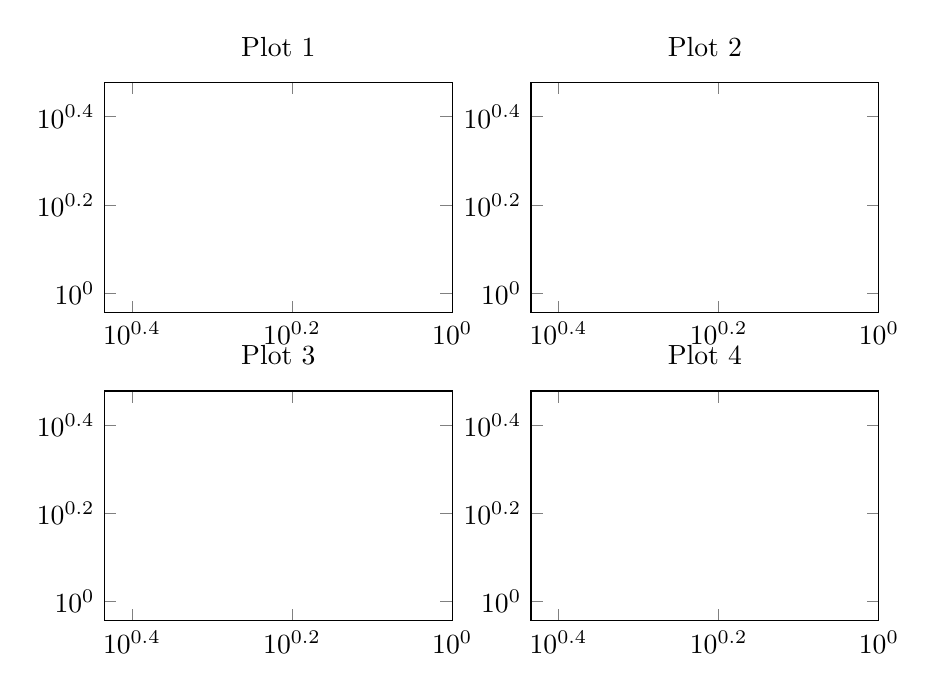
\begin{tikzpicture}

% === Panel 1 (Top Left) ===
\begin{axis}[
    name=plot1,
    width=6cm, height=4.5cm,
    title={Plot 1},
    xmin=10, xmax=4000, xmode=log, x dir=reverse,
    ymode=log,
]
\end{axis}

% === Panel 2 (Top Right) ===
\begin{axis}[
    name=plot2,
    at={(plot1.north east)}, anchor=north west,
    xshift=1cm,                    % spacing between columns
    width=6cm, height=4.5cm,
    title={Plot 2},
    xmin=10, xmax=4000, xmode=log, x dir=reverse,
    ymode=log,
]
\end{axis}

% === Panel 3 (Bottom Left) ===
\begin{axis}[
    name=plot3,
    at={(plot1.south west)}, anchor=north west,
    yshift=-1cm,                   % spacing between rows
    width=6cm, height=4.5cm,
    title={Plot 3},
    xmin=10, xmax=4000, xmode=log, x dir=reverse,
    ymode=log,
]
\end{axis}

% === Panel 4 (Bottom Right) ===
\begin{axis}[
    name=plot4,
    at={(plot3.north east)}, anchor=north west,
    xshift=1cm,
    width=6cm, height=4.5cm,
    title={Plot 4},
    xmin=10, xmax=4000, xmode=log, x dir=reverse,
    ymode=log,
]
\end{axis}

\end{tikzpicture}


\endpgfgraphicnamed


\end{document}

% latex --jobname=g2 grs.tex
% dvips g2.dvi
% dvipdf g2.dvi
